% ecog_coverage.tex -- amsart manuscript.
%
% Every number is a macro from numbers_ecog.tex, generated by
% ../../make_ecog_paper_data.py from ../../results/*.json.  Every figure
% except Fig. 5 is a TikZ/pgfplots source in tikz/, rendered to figures/*.png
% at 600 dpi by build.sh; Fig. 5 is the PyVista render of the repository.
%     cd paper/ecog && ./build.sh
\documentclass[11pt]{amsart}
\usepackage[margin=1in]{geometry}
\usepackage{amssymb,amsthm,mathtools}
\usepackage{graphicx}
\usepackage{booktabs}
\usepackage{microtype}
\usepackage[hidelinks]{hyperref}
\graphicspath{{figures/}}

%% generated by make_ecog_paper_data.py from results/*.json; do not edit
\newcommand{\patchArea}{3777}
\newcommand{\patchVerts}{4977}
\newcommand{\patchTris}{9659}
\newcommand{\patchRadius}{35}
\newcommand{\anchorMNI}{(-58, -38, 38)}
\newcommand{\meshVerts}{175\,409}
\newcommand{\meshTris}{350\,814}
\newcommand{\crownFloor}{12.22}
\newcommand{\crownFloorExact}{12.219}
\newcommand{\crownVerts}{3016}
\newcommand{\crownWorstMNI}{(-51.1, -42.2, 22.1)}
\newcommand{\crownFlatN}{78}
\newcommand{\rhoFreeOne}{35}
\newcommand{\rhoFreeLast}{4.34}
\newcommand{\nMaxGreedy}{160}
\newcommand{\rhoFreeSixtyFour}{6.99}
\newcommand{\rhoCrownSixtyFour}{14.68}
\newcommand{\rhoTwoFreeSixtyFour}{11.50}
\newcommand{\rhoTwoFreeOneTwentyEight}{7.56}
\newcommand{\rhoTwoFreeOneSixty}{6.78}
\newcommand{\minNFourteen}{22}
\newcommand{\minRhoFourteen}{13.25}
\newcommand{\packFourteen}{8}
\newcommand{\diskFailFourteen}{8}
\newcommand{\minNTwelve}{30}
\newcommand{\minRhoTwelve}{11.12}
\newcommand{\packTwelve}{8}
\newcommand{\diskFailTwelve}{10}
\newcommand{\minNTen}{46}
\newcommand{\minRhoTen}{8.88}
\newcommand{\packTen}{12}
\newcommand{\diskFailTen}{32}
\newcommand{\minNEight}{66}
\newcommand{\minRhoEight}{6.95}
\newcommand{\packEight}{16}
\newcommand{\diskFailEight}{24}
\newcommand{\packNine}{13}
\newcommand{\gridUnseenEight}{2082.0}
\newcommand{\gridUnseenPctEight}{55.1}
\newcommand{\gridBettiEight}{(9, 2)}
\newcommand{\gridKEight}{0}
\newcommand{\greedyUnseenEight}{1.0}
\newcommand{\greedyUnseenPctEight}{0.03}
\newcommand{\greedyBettiEight}{(1, 1)}
\newcommand{\greedyKEight}{0}
\newcommand{\greedyQEight}{1}
\newcommand{\gridUnseenTen}{1559.4}
\newcommand{\gridUnseenPctTen}{41.3}
\newcommand{\gridBettiTen}{(6, 1)}
\newcommand{\gridKTen}{0}
\newcommand{\greedyUnseenTen}{0.0}
\newcommand{\greedyUnseenPctTen}{0.00}
\newcommand{\greedyBettiTen}{(1, 0)}
\newcommand{\greedyKTen}{1}
\newcommand{\greedyQTen}{1}
\newcommand{\gridUnseenTwelve}{1079.0}
\newcommand{\gridUnseenPctTwelve}{28.6}
\newcommand{\gridBettiTwelve}{(6, 1)}
\newcommand{\gridKTwelve}{0}
\newcommand{\greedyUnseenTwelve}{0.0}
\newcommand{\greedyUnseenPctTwelve}{0.00}
\newcommand{\greedyBettiTwelve}{(1, 0)}
\newcommand{\greedyKTwelve}{2}
\newcommand{\greedyQTwelve}{3}
\newcommand{\gridSeenPctEight}{45}
\newcommand{\dblAN}{96}
\newcommand{\dblAR}{10}
\newcommand{\dblAOnce}{1.7}
\newcommand{\dblAK}{2}
\newcommand{\dblBN}{112}
\newcommand{\dblBR}{9}
\newcommand{\dblBOnce}{0.0}
\newcommand{\dblBShadow}{(1, 0)}
\newcommand{\dblBMesh}{(1, 1)}
\newcommand{\dblBDisk}{961}
\newcommand{\dblBFaces}{16835}
\newcommand{\offCrownSixtySix}{22}
\newcommand{\offCrownOneTwelve}{31}
\newcommand{\offCrownFortySix}{14}
\newcommand{\offCrownPctLo}{28}
\newcommand{\offCrownPctHi}{33}
\newcommand{\gridPitch}{10}
\newcommand{\gridEuPitchMedian}{9.75}
\newcommand{\gridGeoPitchMedian}{10.24}
\newcommand{\gridGeoPitchOver}{49}
\newcommand{\gridGeoPitchPairs}{112}
\newcommand{\privCountEight}{64}
\newcommand{\privWorstEight}{143.1}
\newcommand{\privMedianEight}{94.2}
\newcommand{\capWholeFiveGridEight}{13.4}
\newcommand{\capWholeTenGridEight}{0.0}
\newcommand{\capTwiceFiveGridEight}{0.0}
\newcommand{\capTwiceTenGridEight}{0.0}
\newcommand{\capMissFiveGridEight}{16.0}
\newcommand{\capMissTenGridEight}{3.7}
\newcommand{\capHiddenGridEight}{13.9}
\newcommand{\capRhoOneGridEight}{21.57}
\newcommand{\capRhoTwoGridEight}{25.02}
\newcommand{\capUnseenGridEight}{2082.0}
\newcommand{\capOnceGridEight}{3297.1}
\newcommand{\capWholeFiveCrownEight}{77.3}
\newcommand{\capWholeTenCrownEight}{47.4}
\newcommand{\capTwiceFiveCrownEight}{10.1}
\newcommand{\capTwiceTenCrownEight}{0.0}
\newcommand{\capMissFiveCrownEight}{0.0}
\newcommand{\capMissTenCrownEight}{0.0}
\newcommand{\capHiddenCrownEight}{4.1}
\newcommand{\capRhoOneCrownEight}{14.68}
\newcommand{\capRhoTwoCrownEight}{15.67}
\newcommand{\capUnseenCrownEight}{223.7}
\newcommand{\capOnceCrownEight}{969.9}
\newcommand{\capWholeFiveFreeSixtyFour}{97.3}
\newcommand{\capWholeTenFreeSixtyFour}{94.0}
\newcommand{\capTwiceFiveFreeSixtyFour}{2.0}
\newcommand{\capTwiceTenFreeSixtyFour}{0.0}
\newcommand{\capMissFiveFreeSixtyFour}{0.0}
\newcommand{\capMissTenFreeSixtyFour}{0.0}
\newcommand{\capHiddenFreeSixtyFour}{0.0}
\newcommand{\capRhoOneFreeSixtyFour}{6.99}
\newcommand{\capRhoTwoFreeSixtyFour}{11.50}
\newcommand{\capUnseenFreeSixtyFour}{1.0}
\newcommand{\capOnceFreeSixtyFour}{923.8}
\newcommand{\capWholeFiveFreeSixtySix}{100.0}
\newcommand{\capWholeTenFreeSixtySix}{100.0}
\newcommand{\capTwiceFiveFreeSixtySix}{2.1}
\newcommand{\capTwiceTenFreeSixtySix}{0.0}
\newcommand{\capMissFiveFreeSixtySix}{0.0}
\newcommand{\capMissTenFreeSixtySix}{0.0}
\newcommand{\capHiddenFreeSixtySix}{0.0}
\newcommand{\capRhoOneFreeSixtySix}{6.95}
\newcommand{\capRhoTwoFreeSixtySix}{10.78}
\newcommand{\capUnseenFreeSixtySix}{0.0}
\newcommand{\capOnceFreeSixtySix}{822.2}
\newcommand{\capWholeFiveGridTen}{28.0}
\newcommand{\capWholeTenGridTen}{2.1}
\newcommand{\capTwiceFiveGridTen}{1.1}
\newcommand{\capTwiceTenGridTen}{0.0}
\newcommand{\capMissFiveGridTen}{8.5}
\newcommand{\capMissTenGridTen}{1.2}
\newcommand{\capHiddenGridTen}{11.7}
\newcommand{\capRhoOneGridTen}{21.57}
\newcommand{\capRhoTwoGridTen}{25.02}
\newcommand{\capUnseenGridTen}{1559.4}
\newcommand{\capOnceGridTen}{2598.9}
\newcommand{\capWholeFiveFreeFortySix}{100.0}
\newcommand{\capWholeTenFreeFortySix}{100.0}
\newcommand{\capTwiceFiveFreeFortySix}{1.1}
\newcommand{\capTwiceTenFreeFortySix}{0.0}
\newcommand{\capMissFiveFreeFortySix}{0.0}
\newcommand{\capMissTenFreeFortySix}{0.0}
\newcommand{\capHiddenFreeFortySix}{0.0}
\newcommand{\capRhoOneFreeFortySix}{8.88}
\newcommand{\capRhoTwoFreeFortySix}{13.71}
\newcommand{\capUnseenFreeFortySix}{0.0}
\newcommand{\capOnceFreeFortySix}{536.9}
\newcommand{\capWholeFiveFreeNinetySix}{100.0}
\newcommand{\capWholeTenFreeNinetySix}{100.0}
\newcommand{\capTwiceFiveFreeNinetySix}{99.6}
\newcommand{\capTwiceTenFreeNinetySix}{99.1}
\newcommand{\capMissFiveFreeNinetySix}{0.0}
\newcommand{\capMissTenFreeNinetySix}{0.0}
\newcommand{\capHiddenFreeNinetySix}{0.0}
\newcommand{\capRhoOneFreeNinetySix}{5.79}
\newcommand{\capRhoTwoFreeNinetySix}{10.09}
\newcommand{\capUnseenFreeNinetySix}{0.0}
\newcommand{\capOnceFreeNinetySix}{1.7}
\newcommand{\capWholeFiveFreeOneTwelve}{100.0}
\newcommand{\capWholeTenFreeOneTwelve}{100.0}
\newcommand{\capTwiceFiveFreeOneTwelve}{100.0}
\newcommand{\capTwiceTenFreeOneTwelve}{100.0}
\newcommand{\capMissFiveFreeOneTwelve}{0.0}
\newcommand{\capMissTenFreeOneTwelve}{0.0}
\newcommand{\capHiddenFreeOneTwelve}{0.0}
\newcommand{\capRhoOneFreeOneTwelve}{5.30}
\newcommand{\capRhoTwoFreeOneTwelve}{8.86}
\newcommand{\capUnseenFreeOneTwelve}{0.0}
\newcommand{\capOnceFreeOneTwelve}{0.0}
\newcommand{\capGridMissZero}{50.9}
\newcommand{\gridHideBound}{13.57}
\newcommand{\dropDraws}{100}
\newcommand{\dropQmax}{8}
\newcommand{\dropMinFreeOneTwelve}{99.9}
\newcommand{\dropMeanOneGridEight}{13.0}
\newcommand{\dropLowOneGridEight}{11.0}
\newcommand{\dropMeanFourGridEight}{11.8}
\newcommand{\dropLowFourGridEight}{8.8}
\newcommand{\dropMeanEightGridEight}{10.1}
\newcommand{\dropLowEightGridEight}{6.5}
\newcommand{\dropMeanOneCrownEight}{75.8}
\newcommand{\dropLowOneCrownEight}{73.1}
\newcommand{\dropMeanFourCrownEight}{70.3}
\newcommand{\dropLowFourCrownEight}{65.1}
\newcommand{\dropMeanEightCrownEight}{62.2}
\newcommand{\dropLowEightCrownEight}{56.3}
\newcommand{\dropMeanOneFreeSixtySix}{96.4}
\newcommand{\dropLowOneFreeSixtySix}{92.6}
\newcommand{\dropMeanFourFreeSixtySix}{86.7}
\newcommand{\dropLowFourFreeSixtySix}{79.2}
\newcommand{\dropMeanEightFreeSixtySix}{74.2}
\newcommand{\dropLowEightFreeSixtySix}{63.1}
\newcommand{\dropMeanOneFreeFortySix}{96.3}
\newcommand{\dropLowOneFreeFortySix}{92.1}
\newcommand{\dropMeanFourFreeFortySix}{87.2}
\newcommand{\dropLowFourFreeFortySix}{81.5}
\newcommand{\dropMeanEightFreeFortySix}{73.9}
\newcommand{\dropLowEightFreeFortySix}{66.1}
\newcommand{\dropMeanOneFreeNinetySix}{100.0}
\newcommand{\dropLowOneFreeNinetySix}{100.0}
\newcommand{\dropMeanFourFreeNinetySix}{100.0}
\newcommand{\dropLowFourFreeNinetySix}{100.0}
\newcommand{\dropMeanEightFreeNinetySix}{99.8}
\newcommand{\dropLowEightFreeNinetySix}{99.4}
\newcommand{\dropMeanOneFreeOneTwelve}{100.0}
\newcommand{\dropLowOneFreeOneTwelve}{100.0}
\newcommand{\dropMeanFourFreeOneTwelve}{99.9}
\newcommand{\dropLowFourFreeOneTwelve}{100.0}
\newcommand{\dropMeanEightFreeOneTwelve}{99.9}
\newcommand{\dropLowEightFreeOneTwelve}{100.0}

% The code release carrying this paper and its Zenodo archive, quoted in the
% Code availability and Acknowledgements.  Release v1.5.0 (tag at commit
% b336049) holds the Python code, results and figure sources of this paper;
% the Lean formalization in lean/ was merged after it.
\newcommand{\codeRepo}{\url{https://github.com/creelie/kshadow-coverage}}
\newcommand{\codeRelease}{v1.5.0}
\newcommand{\zenodoDOI}{10.5281/zenodo.22953062}
%% generated by fold_geometry.py
\def\foldFloorX{41.38}\def\foldFloorY{-14.58}\def\foldRhoC{16.5}
\def\foldNa{9}\def\foldNb{9}\def\foldUnseenPct{33}\def\foldDeep{3}\def\foldR{8}


\newtheorem{theorem}{Theorem}
\newtheorem{proposition}[theorem]{Proposition}
\newtheorem{corollary}[theorem]{Corollary}
\theoremstyle{definition}
\newtheorem{definition}[theorem]{Definition}
\theoremstyle{remark}
\newtheorem{remark}[theorem]{Remark}

\newcommand{\R}{\mathbb{R}}
\DeclareMathOperator{\area}{area}
\newcommand{\dd}{\mathrm{d}}

\title[Optimal ECoG coverage]{Optimal ECoG Coverage\\for Epilepsy Surgery}

\author{Aditi Bose}
\address{Centre for Computational Natural Sciences and Bioinformatics,
International Institute of Information Technology, Hyderabad, India}
\urladdr{https://orcid.org/0000-0002-3036-8223}

\author[D. Bhattacharjee]{Deep Bhattacharjee}
\address{Formerly, Electro-Gravitational Space Propulsion Laboratory (EGSPL),
Bhubaneswar, Odisha 751030, India}
\email{itsdeep@live.com}
\urladdr{https://orcid.org/0000-0003-0466-750X}
\thanks{Deep Bhattacharjee is the corresponding author.}

\author[U. Bhattacharya]{Ushashi Bhattacharya}
\address{Formerly, National Taiwan University, Taipei 106319, Taiwan}
\email{rai.bhattacharya.in@gmail.com}
\urladdr{https://orcid.org/0009-0002-2254-3914}

\date{\today}

\keywords{electrocorticography, epilepsy surgery, seizure onset zone,
electrode placement, covering radius, $k$-fold coverage, nerve theorem}

\begin{document}

\begin{abstract}
Resective surgery can free a patient with drug-resistant focal epilepsy from
seizures. When an intracranial recording guides it, the resection can only be
planned around what the recording's contacts have seen. We treat the placement
of the recording contacts as an optimisation problem on the patient's cortical
surface: every point of the territory suspected of generating the seizures
should lie within a footprint radius $r$ of at least $k$ contacts, measured
along the folded surface. This holds exactly when the $k$-th covering radius
$\rho_k$ of the territory is below $r$, and on a triangulated surface it stays
exact when the covering radius is taken over triangles. An onset zone of any
size and position inside the territory is then seen whole, and it stays seen
whole after any $k-1$ contacts fail. On a $\patchArea$\,mm$^2$ parietal
territory of the colin27 template brain, the documented $8\times8$ subdural
grid leaves $\gridUnseenPctEight\%$ of the territory unseen at $r=8$\,mm, and
an onset zone of radius up to $\capHiddenGridEight$\,mm can lie in it and be
missed entirely. The same 64 contacts placed by covering radius leave
$\greedyUnseenEight$\,mm$^2$ unseen, and $\minNOneEight$ contacts leave
nothing. Contacts confined to the gyral crowns, where a subdural sheet puts
them, cannot reach this at any contact count: counting every crown within
reach, some part of the territory is $\crownFloor$\,mm from its nearest crown.
Covering the territory twice takes $\minNTwoEight$ contacts at $8$\,mm. After
$\dropQmax$ random contact failures these still see a $5$\,mm onset zone whole
in $\dropMeanEightTwoEight\%$ of its possible positions on average, where the
$\minNOneEight$ contacts of single coverage fall to
$\dropMeanEightOneEight\%$. Complete coverage is what lets a resection planned
on the recording contain the onset zone by design; it is not sufficient for
seizure freedom, and this paper reports no patient outcome. We state the
protocol that would test it.
\end{abstract}

\maketitle

% =====================================================================
\section{Introduction}\label{sec:intro}
% =====================================================================

Epilepsy is drug-resistant when two appropriately chosen and tolerated
antiseizure medications have failed~\cite{Kwan2010}, and a substantial
minority of patients reach that point~\cite{KwanBrodie2000}. For focal
drug-resistant epilepsy, resective surgery can end the
seizures~\cite{JobstCascino2015}. For temporal lobe epilepsy, randomised trials found it better than
continued medical therapy~\cite{Wiebe2001,Engel2012}. Its stated goal is
freedom from disabling seizures (Engel class~I) or from all seizures (ILAE
class~1)~\cite{Engel1993,Wieser2001,JobstCascino2015}. Surgery aims at the
epileptogenic zone, the cortex whose removal is needed for seizure freedom,
and when intracranial recording is needed, a central estimate of it is the
seizure onset zone that recording shows~\cite{RosenowLuders2001}.

When the non-invasive evaluation (semiology, scalp video-EEG, MRI, PET, SPECT,
MEG) does not settle where seizures begin, contacts are implanted: subdural
grids and strips for electrocorticography (ECoG), or depth leads for
stereo-EEG~\cite{Jayakar2016,ParviziKastner2018}. The implantation is
hypothesis driven. It samples a territory $X$ that the evaluation says should
contain the onset zone, and what it does not sample it cannot localise
(Fig.~\ref{fig:pathway}). An onset zone that falls between contacts is missed
or truncated, and the resection is then planned around a false or partial
picture, or not at all. Invasive monitoring carries risk: for subdural grids,
complications have been associated with the number of
electrodes~\cite{Hamer2002}, and stereo-EEG has its own complication
profile~\cite{Mullin2016}. The number of contacts cannot simply be raised
until nothing is missed.

\begin{figure}[t]
\centering
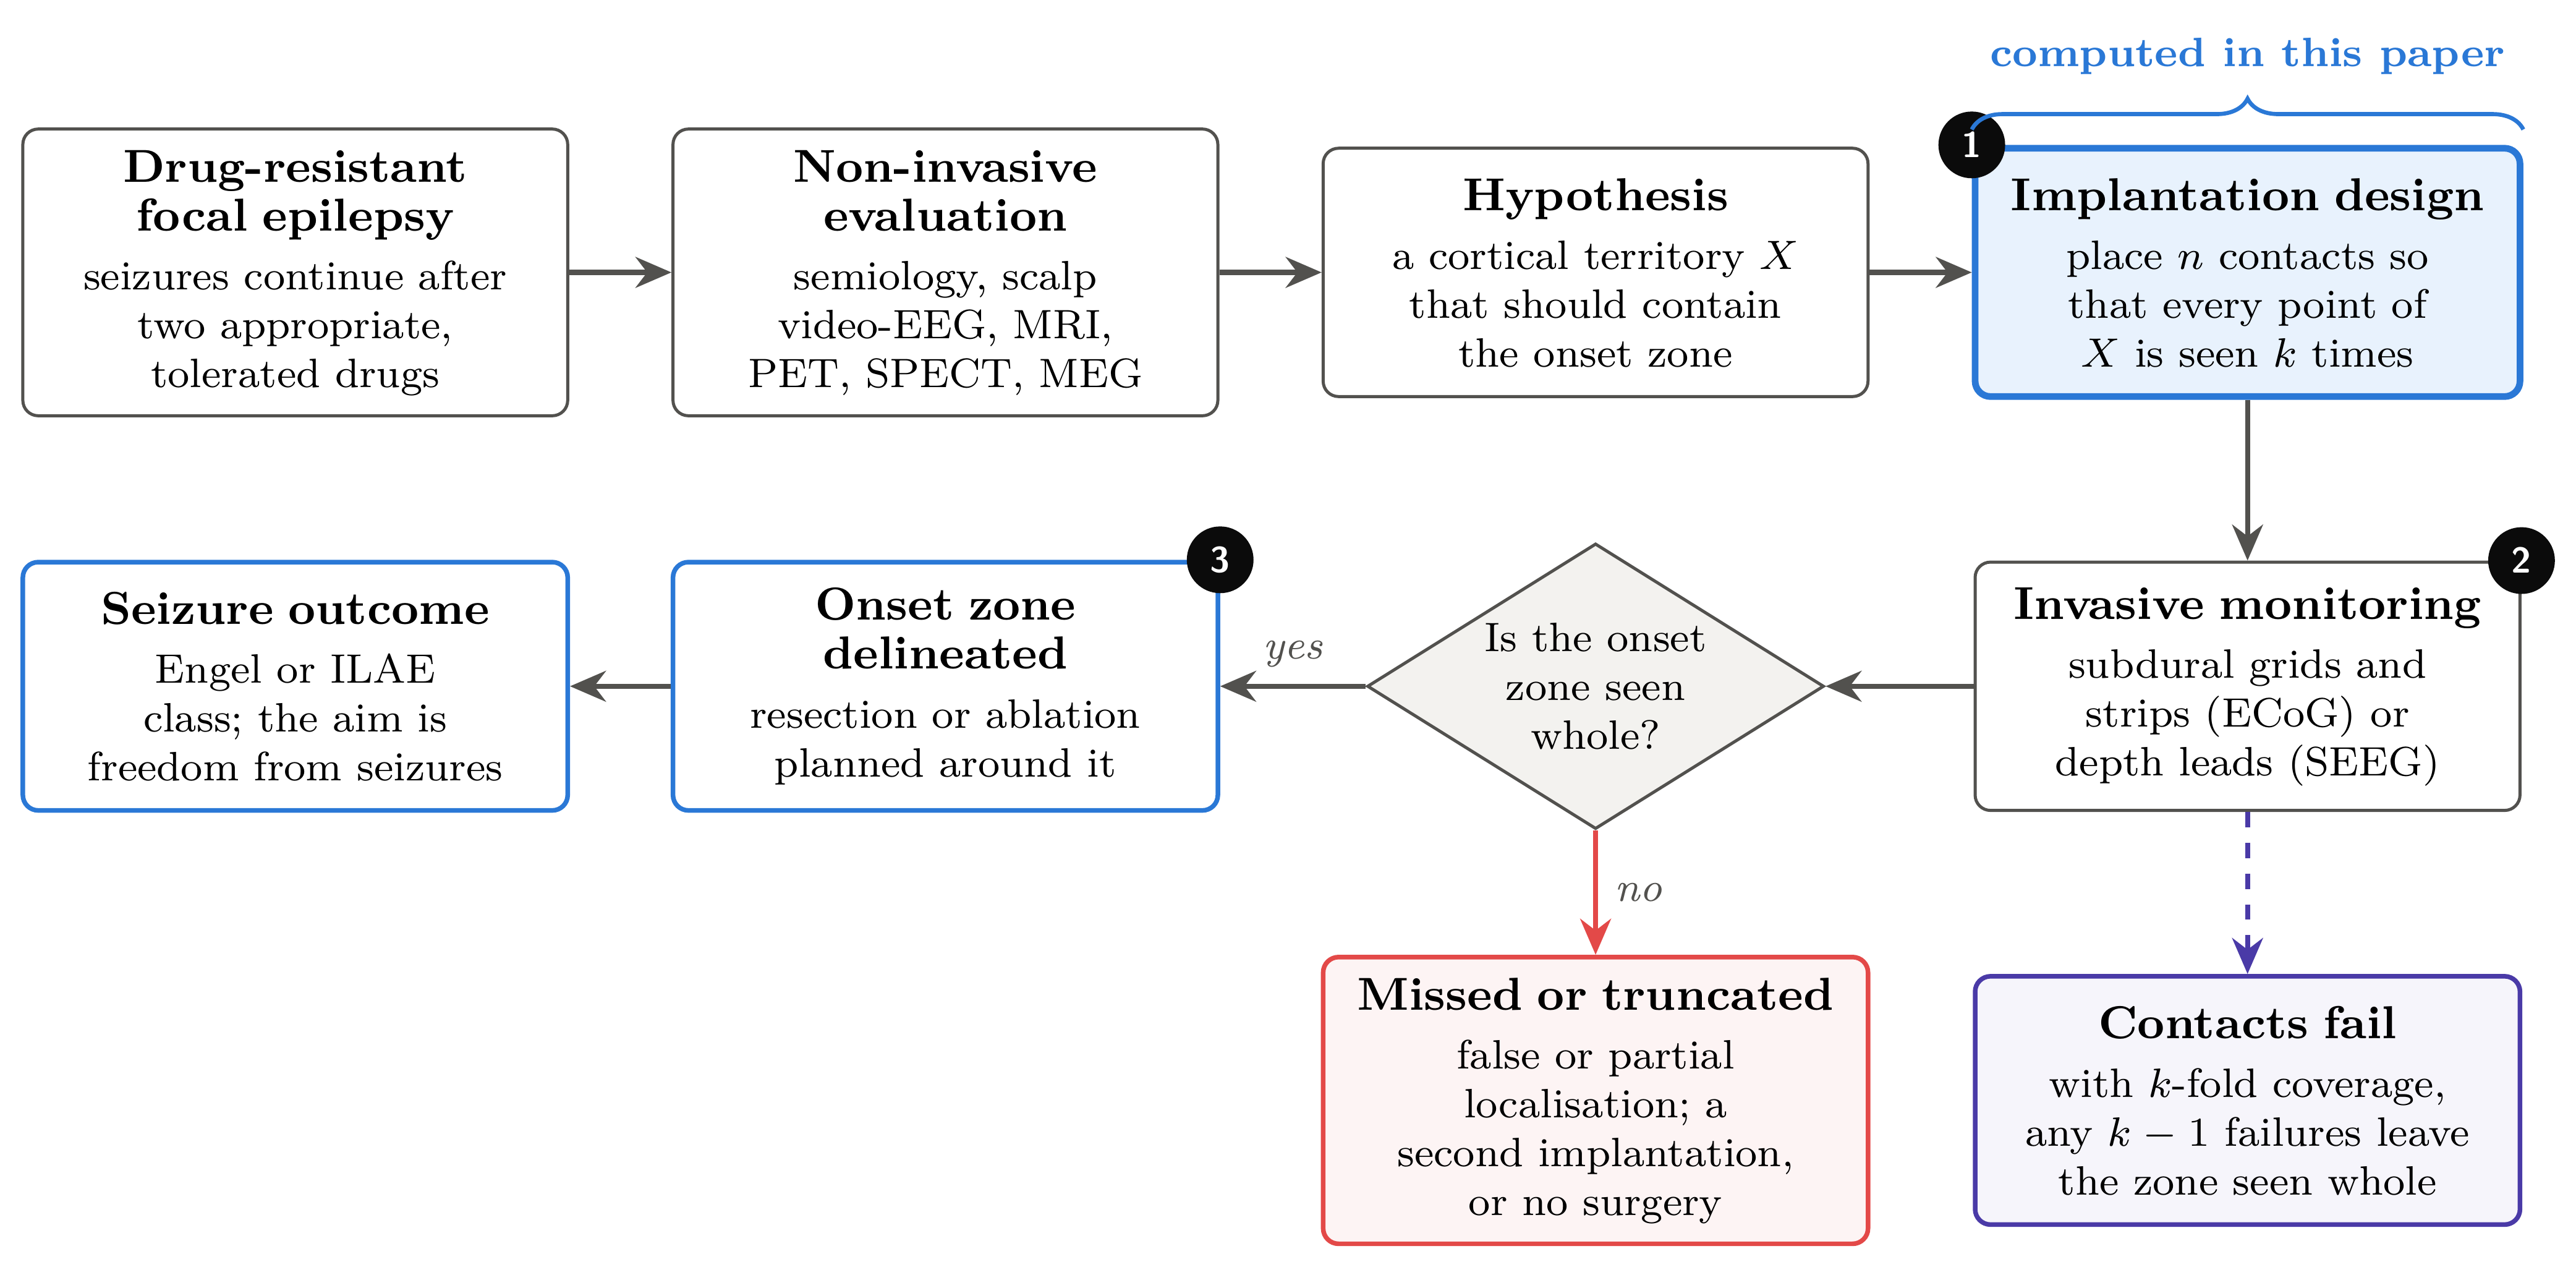
\includegraphics[width=\textwidth]{fig1_pathway.png}
\caption{Where contact placement enters the surgical pathway. The
implantation is designed from a hypothesis, a cortical territory $X$ expected
to contain the seizure onset zone (step 1). What the invasive recording can
localise is limited to what its contacts see (step 2), and a resection aimed at
seizure freedom is planned around the onset zone the recording delineates
(step 3). An onset zone that is missed or seen only in part leads to false or
partial localisation. With $k$-fold coverage, any $k-1$ contact failures during
monitoring leave every onset zone in $X$ seen whole
(Proposition~\ref{prop:failure}). This paper computes step~1.}
\label{fig:pathway}
\end{figure}

This paper asks a narrow question and answers it exactly on the triangulated
surface: given the patient's cortical surface, the territory $X$, and a radius
$r$ within which a contact is credited with recording an onset, where should
$n$ contacts go so that every point of $X$ is seen at least $k$ times, and how
small can $n$ be? The answer turns on one number, the $k$-th covering radius of
$X$ measured along the folded surface (Section~\ref{sec:model}). It gives
three things a clinician can use before implantation. First, a guarantee: when
the covering radius is below $r$, an onset zone of any size and position in
$X$ is seen whole, and stays seen whole after any $k-1$ contacts fail. Second,
a design rule that meets the guarantee; for single coverage with sites anywhere
on $X$ it is provably within a factor of two of the best covering radius for
its contact count, up to one mesh edge. Third, an obstruction: contacts confined to the gyral
crowns, as on a subdural sheet, cannot meet the guarantee below a radius that
is fixed by the folding and not by the number of contacts.

We compute all of this on the colin27 template
brain~\cite{Holmes1998,Oostenveld2011}, where a documented clinical grid
layout~\cite{Stolk2018} can be compared with designed ones, and we extend the
coverage question to the one a surgeon asks: for an onset zone of radius $s$
placed anywhere in $X$, how often is it seen whole, how often is it missed, and
how often does it survive contact failures (Section~\ref{sec:results})?

\subsection*{What this paper does not claim}
Coverage is geometry. Whether a patient becomes seizure-free depends on much
more: whether the onset zone recorded is the epileptogenic zone, whether it
can be resected without unacceptable deficit, and whether the epilepsy is
focal or network-driven~\cite{Spencer2002,Bartolomei2017}. Complete coverage of
the territory is what lets a resection planned on the recording contain the
onset zone by design, not a promise of cure, and incomplete resection of the
recorded onset zone has itself been reported not to predict outcome in one
cohort~\cite{Gascoigne2024}. No patient data and no outcome are used here.
Section~\ref{sec:discussion} states the protocol that would test whether
optimal coverage changes outcome.

\subsection*{Relation to earlier work}
Trajectory planning for stereo-EEG optimises safety and sampling of target
structures~\cite{DeMomi2014,Sparks2017}, electrode spacing has been studied
for how much signal an array resolves~\cite{Slutzky2010}, and
Jaber~et~al.\ test after the fact whether an implantation sampled the
epileptogenic zone~\cite{Jaber2024}. Coverage by sensors with a sensing radius
is classical in sensor networks~\cite{HuangTseng2005}, its topology can be read
from the nerve of the footprints~\cite{Borsuk1948,deSilvaGhrist2007}, and the
$k$-fold region from the multicover nerve~\cite{Sheehy2012}; the certificate
used here as a check follows~\cite{BhattacharjeeBhattacharya2026}. The
placement rule for unrestricted sites is farthest-point sampling, the greedy
algorithm for the $k$-centre problem~\cite{Gonzalez1985,HochbaumShmoys1985}. What is new is the
statement of ECoG placement as a covering-radius problem on the folded
surface, the site floor that it implies for subdural sheets, and the
onset-zone capture and failure analysis of designed arrays. The combinatorial
content of the propositions on the mesh is also proved in the Lean~4 proof
assistant~\cite{deMouraUllrich2021} (Section~\ref{sec:methods}).

% =====================================================================
\section{Coverage of a territory, and of an onset zone}\label{sec:model}
% =====================================================================

Let $M$ be the patient's pial surface, a closed surface with the geodesic
distance $\dd$ (the length of the shortest path along the surface). Let
$X\subseteq M$ be the target territory, a compact region; $C\subseteq M$ the
sites a contact may occupy; and $P=\{p_1,\dots,p_n\}\subseteq C$ the contacts.
A contact sees the points within distance $r$ of it along the surface; its
footprint is $B_i=\{x\in M:\dd(x,p_i)<r\}$. The multiplicity of a point is
$m(x)=\#\{i:x\in B_i\}$, and the region seen at least $k$ times is
$R_k=\{x:m(x)\ge k\}$, so that $R_1\supseteq R_2\supseteq\cdots$
(Fig.~\ref{fig:model}).

\begin{definition}
For $x\in M$ let $\dd_k(x,P)$ be the distance from $x$ to its $k$-th nearest
contact. The \emph{$k$-th covering radius} of $X$ by $P$ is
\[
\rho_k(P)=\max_{x\in X}\dd_k(x,P).
\]
\end{definition}

\begin{proposition}[coverage is a covering radius]\label{prop:cover}
$X\subseteq R_k$ if and only if $\rho_k(P)<r$.
\end{proposition}

\begin{proof}
A point $x$ lies in $R_k$ exactly when at least $k$ contacts are within
distance less than $r$ of it, that is, when $\dd_k(x,P)<r$. This holds for
every $x\in X$ exactly when it holds for a maximiser of $\dd_k(\cdot,P)$ on
$X$, which exists because $\dd_k(\cdot,P)$ is continuous and $X$ is compact.
\end{proof}

So the whole design problem is to push $\rho_k(P)$ below $r$ with as few
contacts as possible.

\subsection*{Onset zones and contact failure}
An onset zone is a region $Z\subseteq X$ of unknown position. We say $Z$ is
\emph{seen whole} if $Z\subseteq R_1$, and \emph{missed} if $Z\cap
R_1=\emptyset$. Contacts fail during monitoring, through lost contact with the
cortex, noise or artefact, and the question is whether $Z$ is still seen whole
by the contacts that remain.

\begin{proposition}[failure-proof sampling]\label{prop:failure}
Let $Z\subseteq X$ and $q\ge0$. Every set of at most $q$ failed contacts leaves
$Z$ seen whole by the survivors if and only if $Z\subseteq R_{q+1}$. In
particular, if $\rho_{q+1}(P)<r$, every onset zone in $X$, of any size and
position, is seen whole after any $q$ contacts fail.
\end{proposition}

\begin{proof}
If $Z\subseteq R_{q+1}$, a point $x\in Z$ lies in at least $q+1$ footprints,
at most $q$ of which have failed, so a surviving footprint contains $x$.
Conversely, if some $x\in Z$ has $m(x)\le q$, let the $m(x)$ contacts whose
footprints contain $x$ fail; that is at most $q$ failures, and $x$ is no longer
seen. The last sentence follows from Proposition~\ref{prop:cover} with
$k=q+1$.
\end{proof}

The guarantee is worst case: it holds for every failure set, however
unlucky, not merely on average. Section~\ref{sec:results} also measures the
average under random failure.

\subsection*{Capture of an onset zone of given size}
When $X\not\subseteq R_k$ the answer depends on the size and position of the
onset zone. Model it as the closed geodesic disk
$Z_s(x)=\{y:\dd(x,y)\le s\}$ of radius $s$ about a centre $x$, admissible when
$Z_s(x)\subseteq X$, and let $A_s$ be the set of admissible centres. With
$\mu$ the area measure, define, for every $s$ with $\mu(A_s)>0$,
\[
W_k(s)=\frac{\mu\{x\in A_s:Z_s(x)\subseteq R_k\}}{\mu(A_s)},\qquad
L(s)=\frac{\mu\{x\in A_s:Z_s(x)\cap R_1=\emptyset\}}{\mu(A_s)}.
\]
If the centre of the onset zone is equally likely to be anywhere it fits in
$X$, $W_1(s)$ is the probability that the array sees it whole, $W_2(s)$ the
probability that it still does after any one failure, and $L(s)$ the
probability that it is missed entirely. The uniform prior is an assumption of
the model. With a patient-specific prior, for instance from the concordance of
non-invasive tests, $\mu$ is replaced by that prior and nothing else changes.

\begin{proposition}[capture by erosion]\label{prop:erosion}
$Z_s(x)\subseteq R_k$ if and only if $\dd(x,M\setminus R_k)>s$. For $s>0$,
$Z_s(x)\cap R_1=\emptyset$ if and only if $\dd(x,R_1)\ge s$; for $s=0$, if
and only if $x\notin R_1$. Consequently, for every $s$ with $\mu(A_s)>0$:
\begin{enumerate}
\item if $X\subseteq R_k$ then $W_k(s)=1$ and $L(s)=0$, and
$W_k(0)=\mu(X\cap R_k)/\mu(X)$ in general;
\item with $h(P)=\max_{x\in X}\min\{\dd(x,R_1),\,\dd(x,M\setminus X)\}$,
$L(s)>0$ if $s<h(P)$ and $L(s)=0$ if $s>h(P)$: $h(P)$ is the radius of the
largest onset zone the array can miss entirely. Moreover
\[
h(P)\ \ge\ \max_{x\in X}\min\{\dd_1(x,P)-r,\ \dd(x,M\setminus X)\}.
\]
\end{enumerate}
\end{proposition}

\begin{proof}
The set $M\setminus R_k$ is closed, so it avoids the closed disk $Z_s(x)$
exactly when its distance from $x$ exceeds $s$. The set $R_1$ is open. Let
$s>0$: if $\dd(x,R_1)\ge s$ and some $y\in R_1$ had $\dd(x,y)\le s$, then
$\dd(x,y)=s>0$, and points of a shortest path from $x$ to $y$ close to $y$
would lie in $R_1$ at distance less than $s$; so $Z_s(x)\cap R_1=\emptyset$
exactly when $\dd(x,R_1)\ge s$. The same argument with the open set
$M\setminus X$ shows that, for $s>0$, $x$ is admissible exactly when
$\dd(x,M\setminus X)\ge s$, while $A_0=X$. For (1),
if $X\subseteq R_k$ every admissible disk lies in $R_k$ and meets $R_1$; and
$A_0=X$, $Z_0(x)=\{x\}$. For (2), if $s<h(P)$ the set of $x$ with
$\dd(x,R_1)>s$ and $\dd(x,M\setminus X)>s$ is open, by continuity of both
distances, and nonempty, so it has positive area, and each of its points is an
admissible centre whose disk is missed; if $s>h(P)$ no admissible centre has
$\dd(x,R_1)\ge s$. For the bound, if $y\in R_1$ then $\dd(y,p)<r$ for some
contact $p$, so $\dd(x,y)\ge\dd(x,p)-r\ge\dd_1(x,P)-r$.
\end{proof}

Each of $W_k$ and $L$ is therefore one multi-source Dijkstra
run~\cite{Dijkstra1959}, from the unseen set or from the seen set, followed by
a threshold at each $s$. Part (2) turns the covering radius into a clinical
statement: an array whose covering radius exceeds the footprint by $\delta$ at
a point at least $\delta$ inside $X$ can miss an onset zone of radius about
$\delta$ there entirely, whatever else it records.

\subsection*{On the triangulated surface}
Every computation is done on the triangle mesh of the pial surface, and the
definitions have to be carried over in a way that keeps the propositions
exact. We take triangles as the atoms. Distances are shortest paths on the
edge graph of the mesh. The distance from a contact $p$ to a triangle $T$ is
the distance to its farthest vertex, $e(p,T)=\max_{v\in T}\dd(v,p)$, and $T$
lies in the footprint of $p$ when $e(p,T)<r$, so that a triangle counts as seen
only when a single contact sees all of it. $R_k$ is the set of triangles in at
least $k$ footprints, and the $k$-th covering radius is
$\rho_k(P)=\max_{T\in X}\bigl(\text{$k$-th smallest of }e(p,T)\text{ over }p\in
P\bigr)$. The onset zone about a triangle $T_0$ of $X$ is the set of triangles
whose centroids lie within distance $s$ of the centroid of $T_0$, distances
now running on the edge graph with every centroid joined to the vertices of
its triangle; $\mu$ is triangle area. With these definitions
Propositions~\ref{prop:cover}--\ref{prop:erosion} hold on the mesh with the
same proofs, reading triangles for points, both conditions of
Proposition~\ref{prop:erosion} as strict inequalities between finite distances,
and $W_k(0)=\mu(X\cap R_k)/\mu(X)$ exactly; the lower bound on $h(P)$ is a
statement about the continuous surface.

The triangle rule is conservative, and the choice matters in practice. The
vertex covering radius $\rho_k^{\mathrm{v}}(P)=\max_{v\in X}\dd_k(v,P)$, taken
over the vertices of $X$ alone, satisfies
\[
\rho_k^{\mathrm{v}}(P)\ \le\ \rho_k(P)\ \le\ \rho_k^{\mathrm{v}}(P)+\ell,
\]
where $\ell$ is the longest edge of $X$ ($\edgeMax$\,mm here, median
$\edgeMedian$\,mm), because $e(p,T)\le\dd(v,p)+\ell$ for every vertex $v$ of
$T$. It can therefore fall below $r$ while a triangle is still unseen: 64
contacts placed by farthest-point sampling have $\rho_1^{\mathrm{v}}=
\rhoFreeSixtyFourVertex$\,mm but $\rho_1=\rhoFreeSixtyFour$\,mm, and at
$r=8$\,mm they leave $\greedyUnseenEight$\,mm$^2$ unseen
(Section~\ref{sec:results}).

\subsection*{The shape of the covered region}
Where coverage is not complete, its shape matters. A hole in $R_1$, a pocket of
unseen cortex surrounded by seen cortex, is exactly where an onset zone can
hide while every contact around it records (Fig.~\ref{fig:model}a). The
topology of $R_k$ can be read from which footprints overlap: when every
nonempty intersection of footprints is contractible, $R_k$ is homotopy
equivalent to the $k$-shadow of the nerve of the
footprints~\cite{Sheehy2012,BhattacharjeeBhattacharya2026}, whose Betti numbers
$(b_0,b_1)$ count pieces and holes. We use this certificate as an independent
check on every design, on the understanding established in
earlier work~\cite{kshadowcode}: geodesic footprints on a folded cortex are
not always convex, so the certificate is checked against a direct computation
on the mesh, and a certificate of $(1,0)$ says that $R_k$ is one piece without
holes, not that it contains $X$. Containment is decided by
Proposition~\ref{prop:cover}.

\begin{figure}[t]
\centering
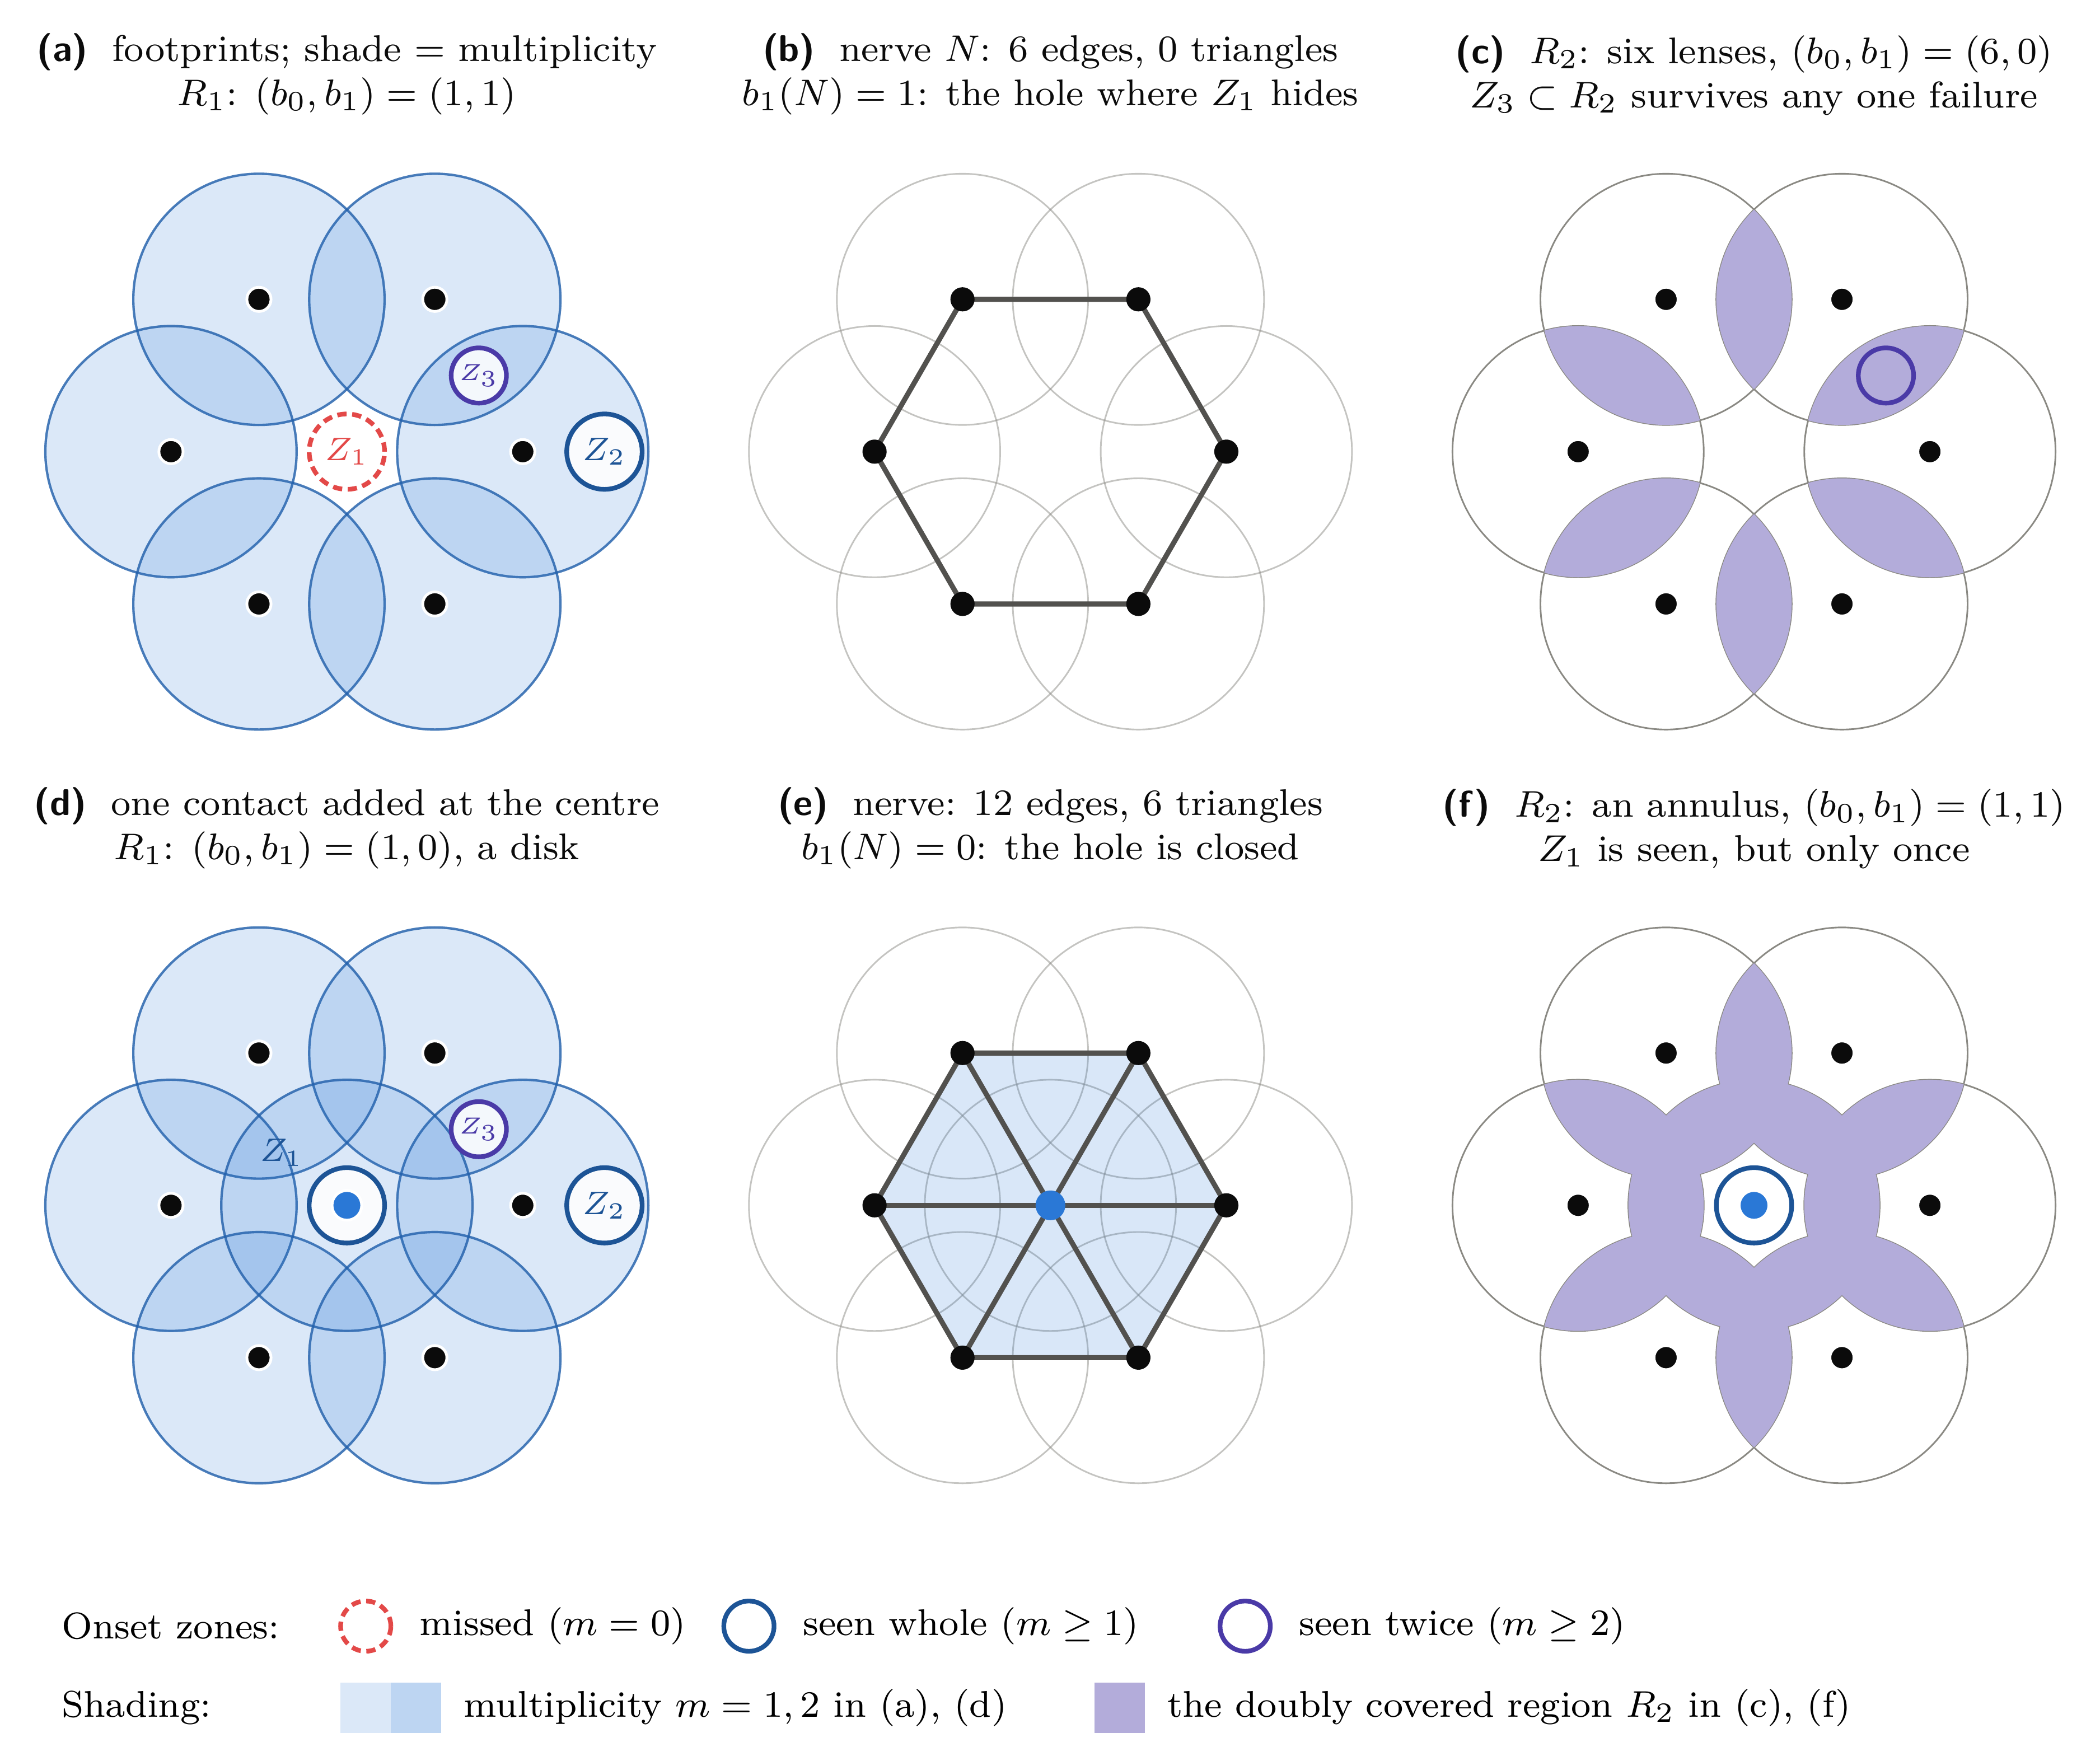
\includegraphics[width=\textwidth]{fig2_model.png}
\caption{Footprints, the nerve, and what they say about an onset zone. Six
contacts on a ring, footprints of radius $1$ (top), and the same with one
contact added at the centre (bottom). (a) The multiplicity $m$ of the
footprints. $R_1$ has a hole, and an onset zone $Z_1$ inside it is missed
although six contacts surround it; $Z_2$ is seen whole once; $Z_3$ lies where
two footprints overlap. (b) The nerve: an edge for each pair of overlapping
footprints, a triangle for each triple with a common point. Its cycle is the
hole of (a), found from overlaps alone. (c) The doubly covered region $R_2$,
six lenses; $Z_3\subset R_2$ is still seen whole if any one contact fails
(Proposition~\ref{prop:failure}). (d)--(f) One contact added at the centre
closes the hole: $Z_1$ is now seen, but only once, since $R_2$ is an annulus
around it. Every statement in the panel titles was checked numerically.}
\label{fig:model}
\end{figure}

% =====================================================================
\section{Why a subdural sheet cannot reach the folds}\label{sec:floor}
% =====================================================================

A subdural grid is a flat sheet laid on the surface of the brain. Its contacts
sit on the gyral crowns; the banks and fundi of the sulci can lie a centimetre
or more of cortex away along the surface, however close they are in a
straight line (Fig.~\ref{fig:fold}). Three elementary facts make this exact
and say what can be done instead. The first holds for any $k$; take $C$ finite
(on a mesh, a set of vertices) and $P$ a set of distinct sites of $C$.

\begin{proposition}[site floor]\label{prop:sitefloor}
Put $\rho_C^{(k)}=\max_{x\in X}\dd_k(x,C)$, the distance from $x$ to its $k$-th
nearest site of $C$, maximised over $X$, and $\rho_C=\rho_C^{(1)}$. Then
$\rho_k(P)\ge\rho_C^{(k)}$ for every $P\subseteq C$. So if $r\le\rho_C^{(k)}$,
no array with its contacts in $C$ sees all of $X$ $k$ times, at any number of
contacts.
\end{proposition}

\begin{proof}
Since $P\subseteq C$, the $k$ nearest contacts of any $x$ are among its sites
in $C$, so $\dd_k(x,P)\ge\dd_k(x,C)$; take $x$ attaining $\rho_C^{(k)}$. The
second sentence is Proposition~\ref{prop:cover}. On the mesh the same argument
applies to $e(\cdot,T)$ triangle by triangle.
\end{proof}

\begin{proposition}[packing bound]\label{prop:packing}
If $S\subseteq X$ has $\dd(s,s')\ge 2r$ for all distinct $s,s'\in S$, then
every array with $X\subseteq R_1$ has at least $|S|$ contacts.
\end{proposition}

\begin{proof}
If $s$ and $s'$ lay in one footprint $B(p,r)$, then $\dd(s,s')\le
\dd(s,p)+\dd(p,s')<2r$. So each footprint contains at most one point of $S$,
and the footprints cover $S$. On the mesh take $S$ a set of vertices of $X$:
each lies in a seen triangle and so within $r$ of the contact that sees it.
\end{proof}

\begin{proposition}[farthest-point placement is within a factor two]
\label{prop:greedy}
On a mesh, let $p_1,p_2,\dots$ be vertices of $X$, each $p_{j+1}$ a vertex of
$X$ farthest from $P_j=\{p_1,\dots,p_j\}$. Then for every $n$ and every set $Q$
of $n$ vertices of $M$, $\rho_1^{\mathrm{v}}(P_n)\le2\rho_1^{\mathrm{v}}(Q)$, and
$\rho_1(P_n)\le2\rho_1(Q)+\ell$.
\end{proposition}

\begin{proof}
Since $p_{j+1}$ is a farthest vertex of $X$ from $P_j$,
$\dd(p_{j+1},P_j)=\rho_1^{\mathrm{v}}(P_j)$, and $\rho_1^{\mathrm{v}}(P_j)$
does not increase with $j$. So any two of $p_1,\dots,p_{n+1}$ are at least
$\rho_1^{\mathrm{v}}(P_n)$ apart. Send each of these $n+1$ points to its
nearest point of $Q$; two of them, $p_i$ and $p_j$, share a nearest point $q$,
and $\rho_1^{\mathrm{v}}(P_n)\le\dd(p_i,p_j)\le\dd(p_i,q)+\dd(q,p_j)\le
2\rho_1^{\mathrm{v}}(Q)$. The second inequality follows from the first and
the bounds between $\rho_1^{\mathrm{v}}$ and $\rho_1$.
\end{proof}

Proposition~\ref{prop:sitefloor} is the obstruction.
Proposition~\ref{prop:packing} bounds the contact count from below, and
Proposition~\ref{prop:greedy} says the placement rule we use loses at most a
factor two in radius, up to one mesh edge, against any placement with the same
number of contacts. On a surface the count scales like the inverse square of
the radius, so the factor two in radius becomes about four in contact count.
The guarantee is for single coverage with sites anywhere on $X$. For $k\ge2$
the same rule, and for sites restricted to $C$ the worst-triangle rule of
Section~\ref{sec:design}, are heuristics, and their designs are checked by
Proposition~\ref{prop:cover} rather than bounded in advance.

\begin{figure}[t]
\centering
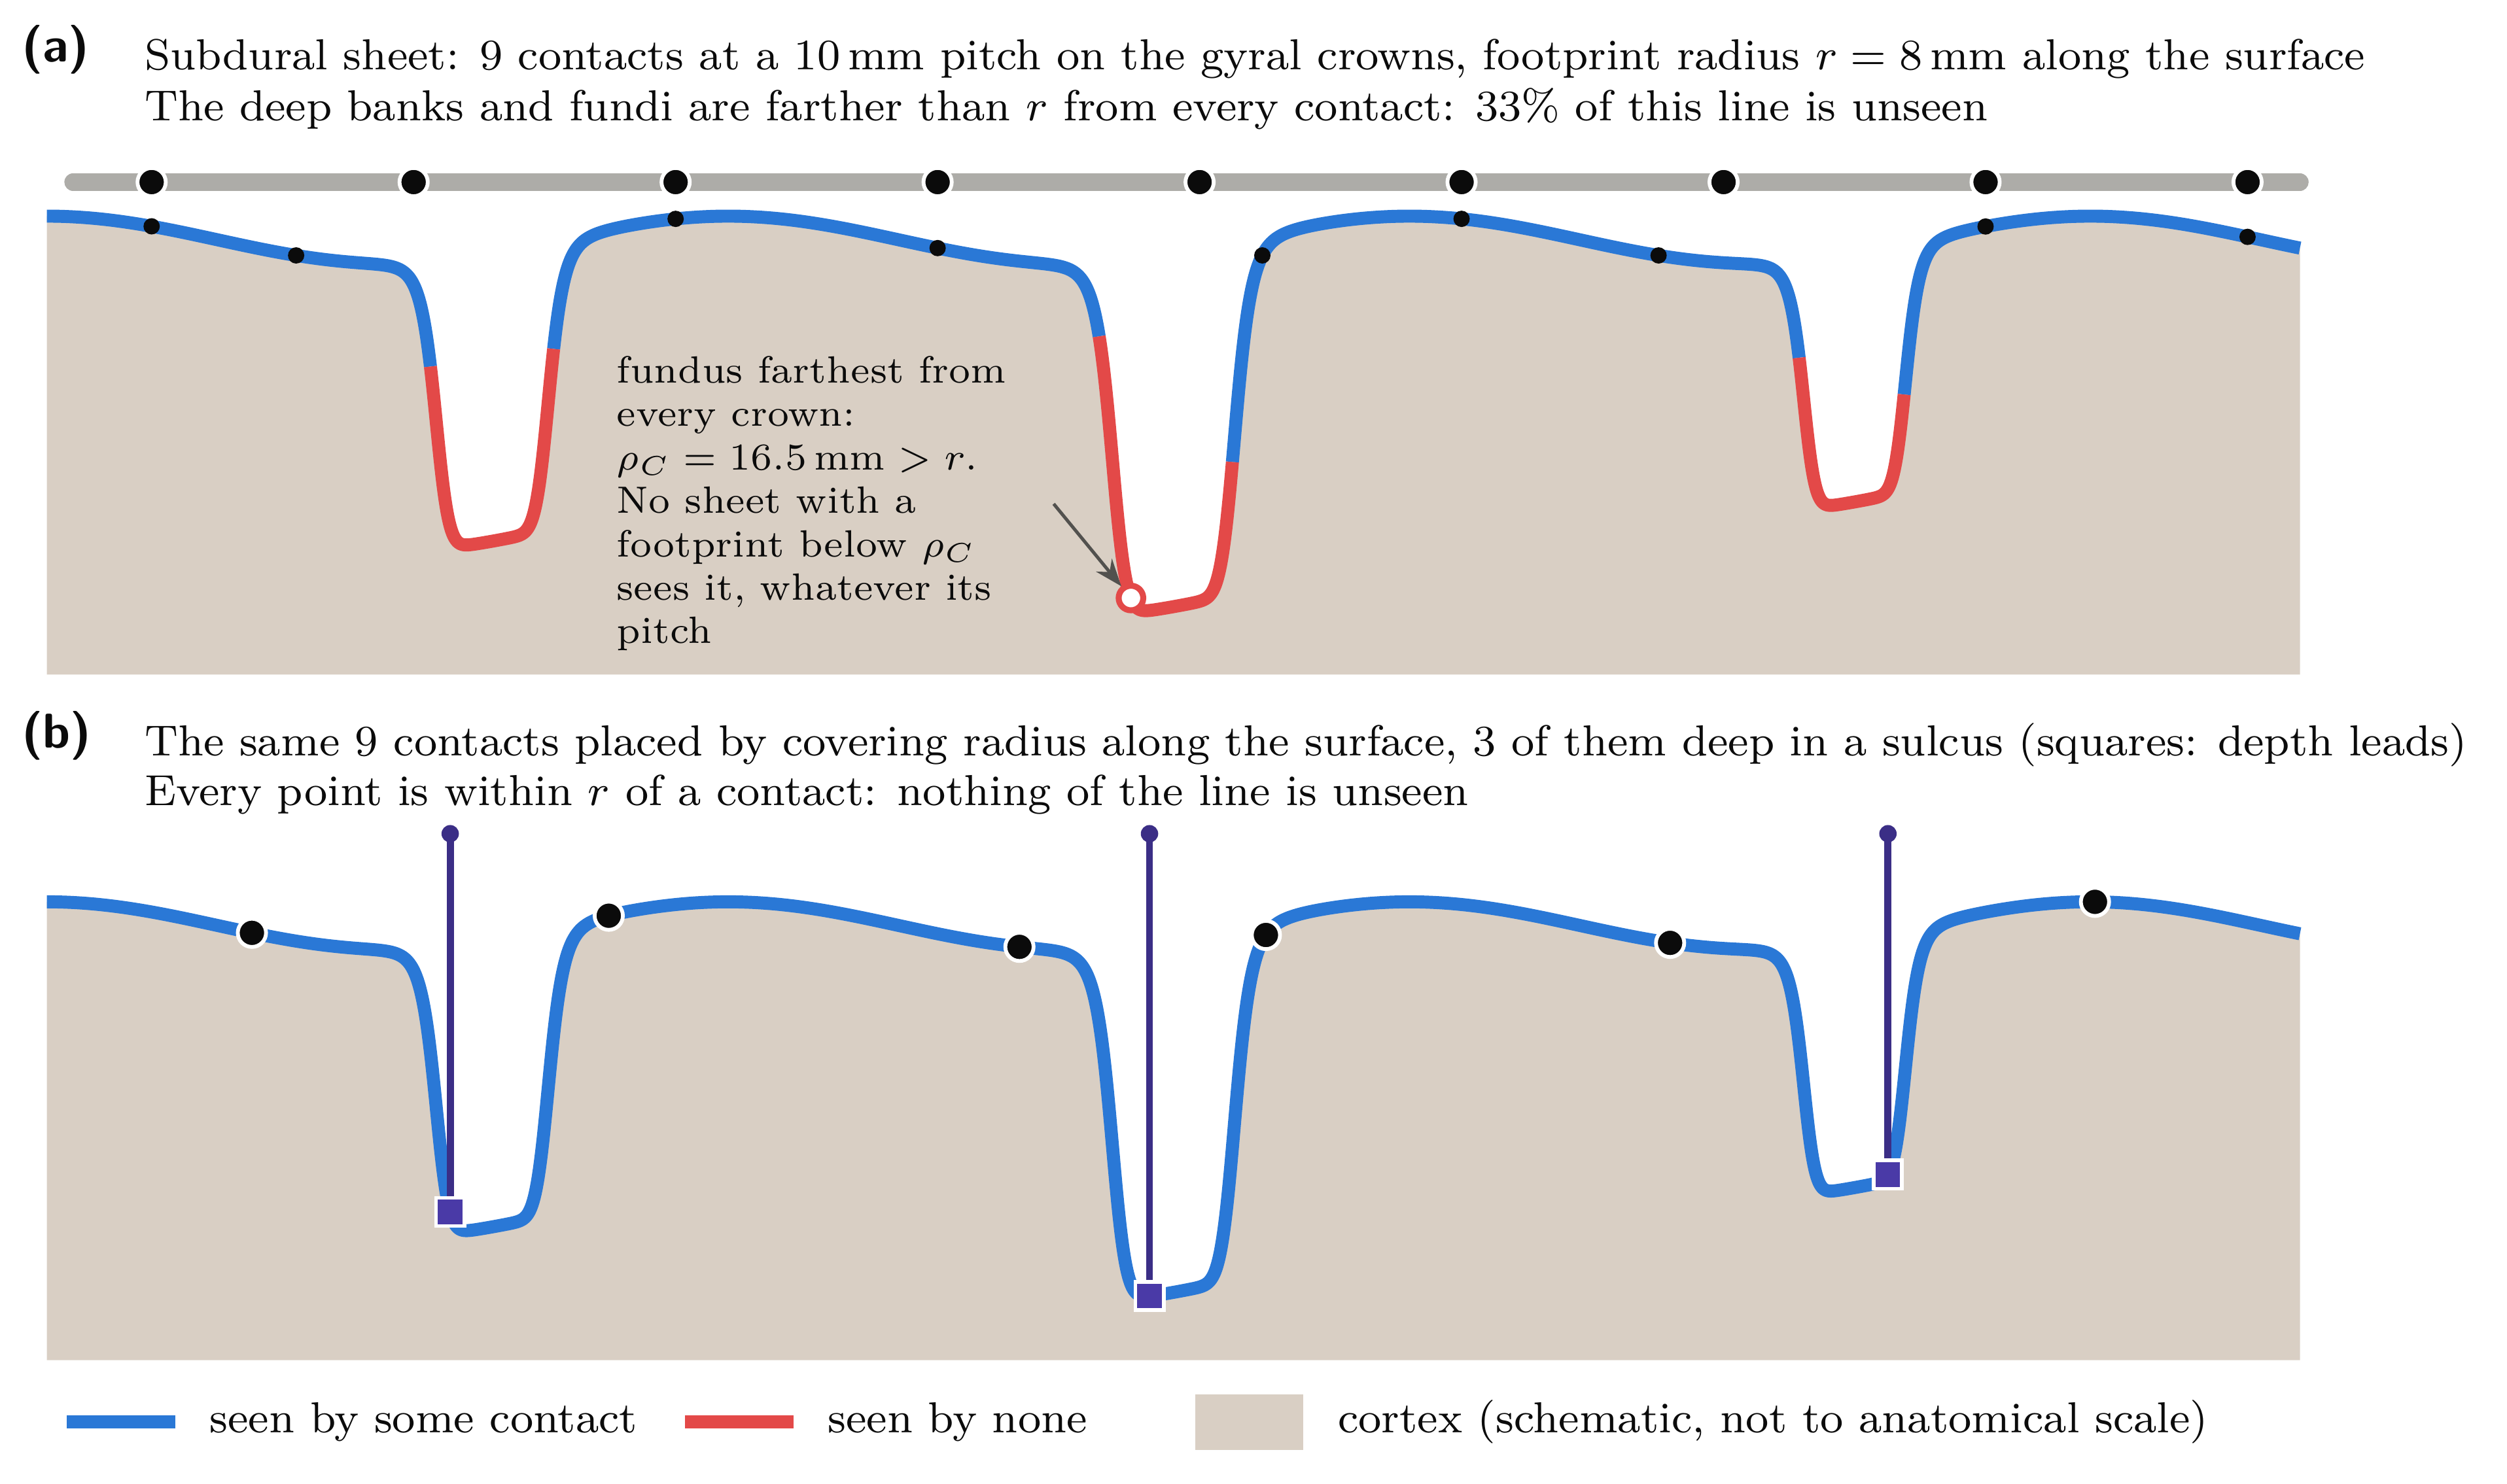
\includegraphics[width=\textwidth]{fig3_fold.png}
\caption{The site floor in one cross-section (schematic; distances are arc
length along the pial line). (a) A subdural sheet with $\foldNa$ contacts at a
$10$\,mm pitch; large dots are contacts on the sheet and small dots the crown
points they rest on. With footprint radius $r=\foldR$\,mm the deep banks and
fundi are seen by no contact, $\foldUnseenPct\%$ of the line. The fundus
marked is the point farthest from the crowns: its nearest crown point is
$\rho_C=\foldRhoC$\,mm away, so no sheet with a footprint radius below that
sees it, at any pitch (Proposition~\ref{prop:sitefloor}). (b) The same
$\foldNb$ contacts placed by covering radius along the line, $\foldDeep$ of
them deep in a sulcus on depth leads: every point is within $r$ of a contact.
Geometry from \texttt{tikz/fold\_geometry.py}.}
\label{fig:fold}
\end{figure}

% =====================================================================
\section{Designing the array}\label{sec:design}
% =====================================================================

The design procedure follows from Section~\ref{sec:model} and is summarised
in Fig.~\ref{fig:algorithm}. Given $M$, $X$, $C$, $r$ and $k$: compute the
site floor $\rho_C^{(k)}$ over every admissible site that can reach $X$. If
$\rho_C^{(k)}\ge r$ the sites are infeasible (Proposition~\ref{prop:sitefloor}),
and $C$ has to be enlarged, with depth leads or strips placed into the sulci,
or a larger radius accepted. Otherwise add contacts one at a time, updating
$\rho_1,\dots,\rho_k$ exactly after each, until $\rho_k<r$: when sites may be
anywhere on $X$, by farthest-point sampling; when they are restricted to $C$,
by adding the site of $C$ closest, in $e(c,T)$, to the worst covered triangle
of $X$; by Proposition~\ref{prop:cover} the design then sees all of $X$
$k$ times, on the mesh and triangle by triangle. Then report the certificate of
the covered region with its disk test, and the capture curves $W_1$, $W_k$ and
$L$. The procedure needs the patient's pial surface, which can be
reconstructed from the presurgical MRI with standard
tools~\cite{Dale1999,Fischl2012}.

\begin{figure}[t]
\centering
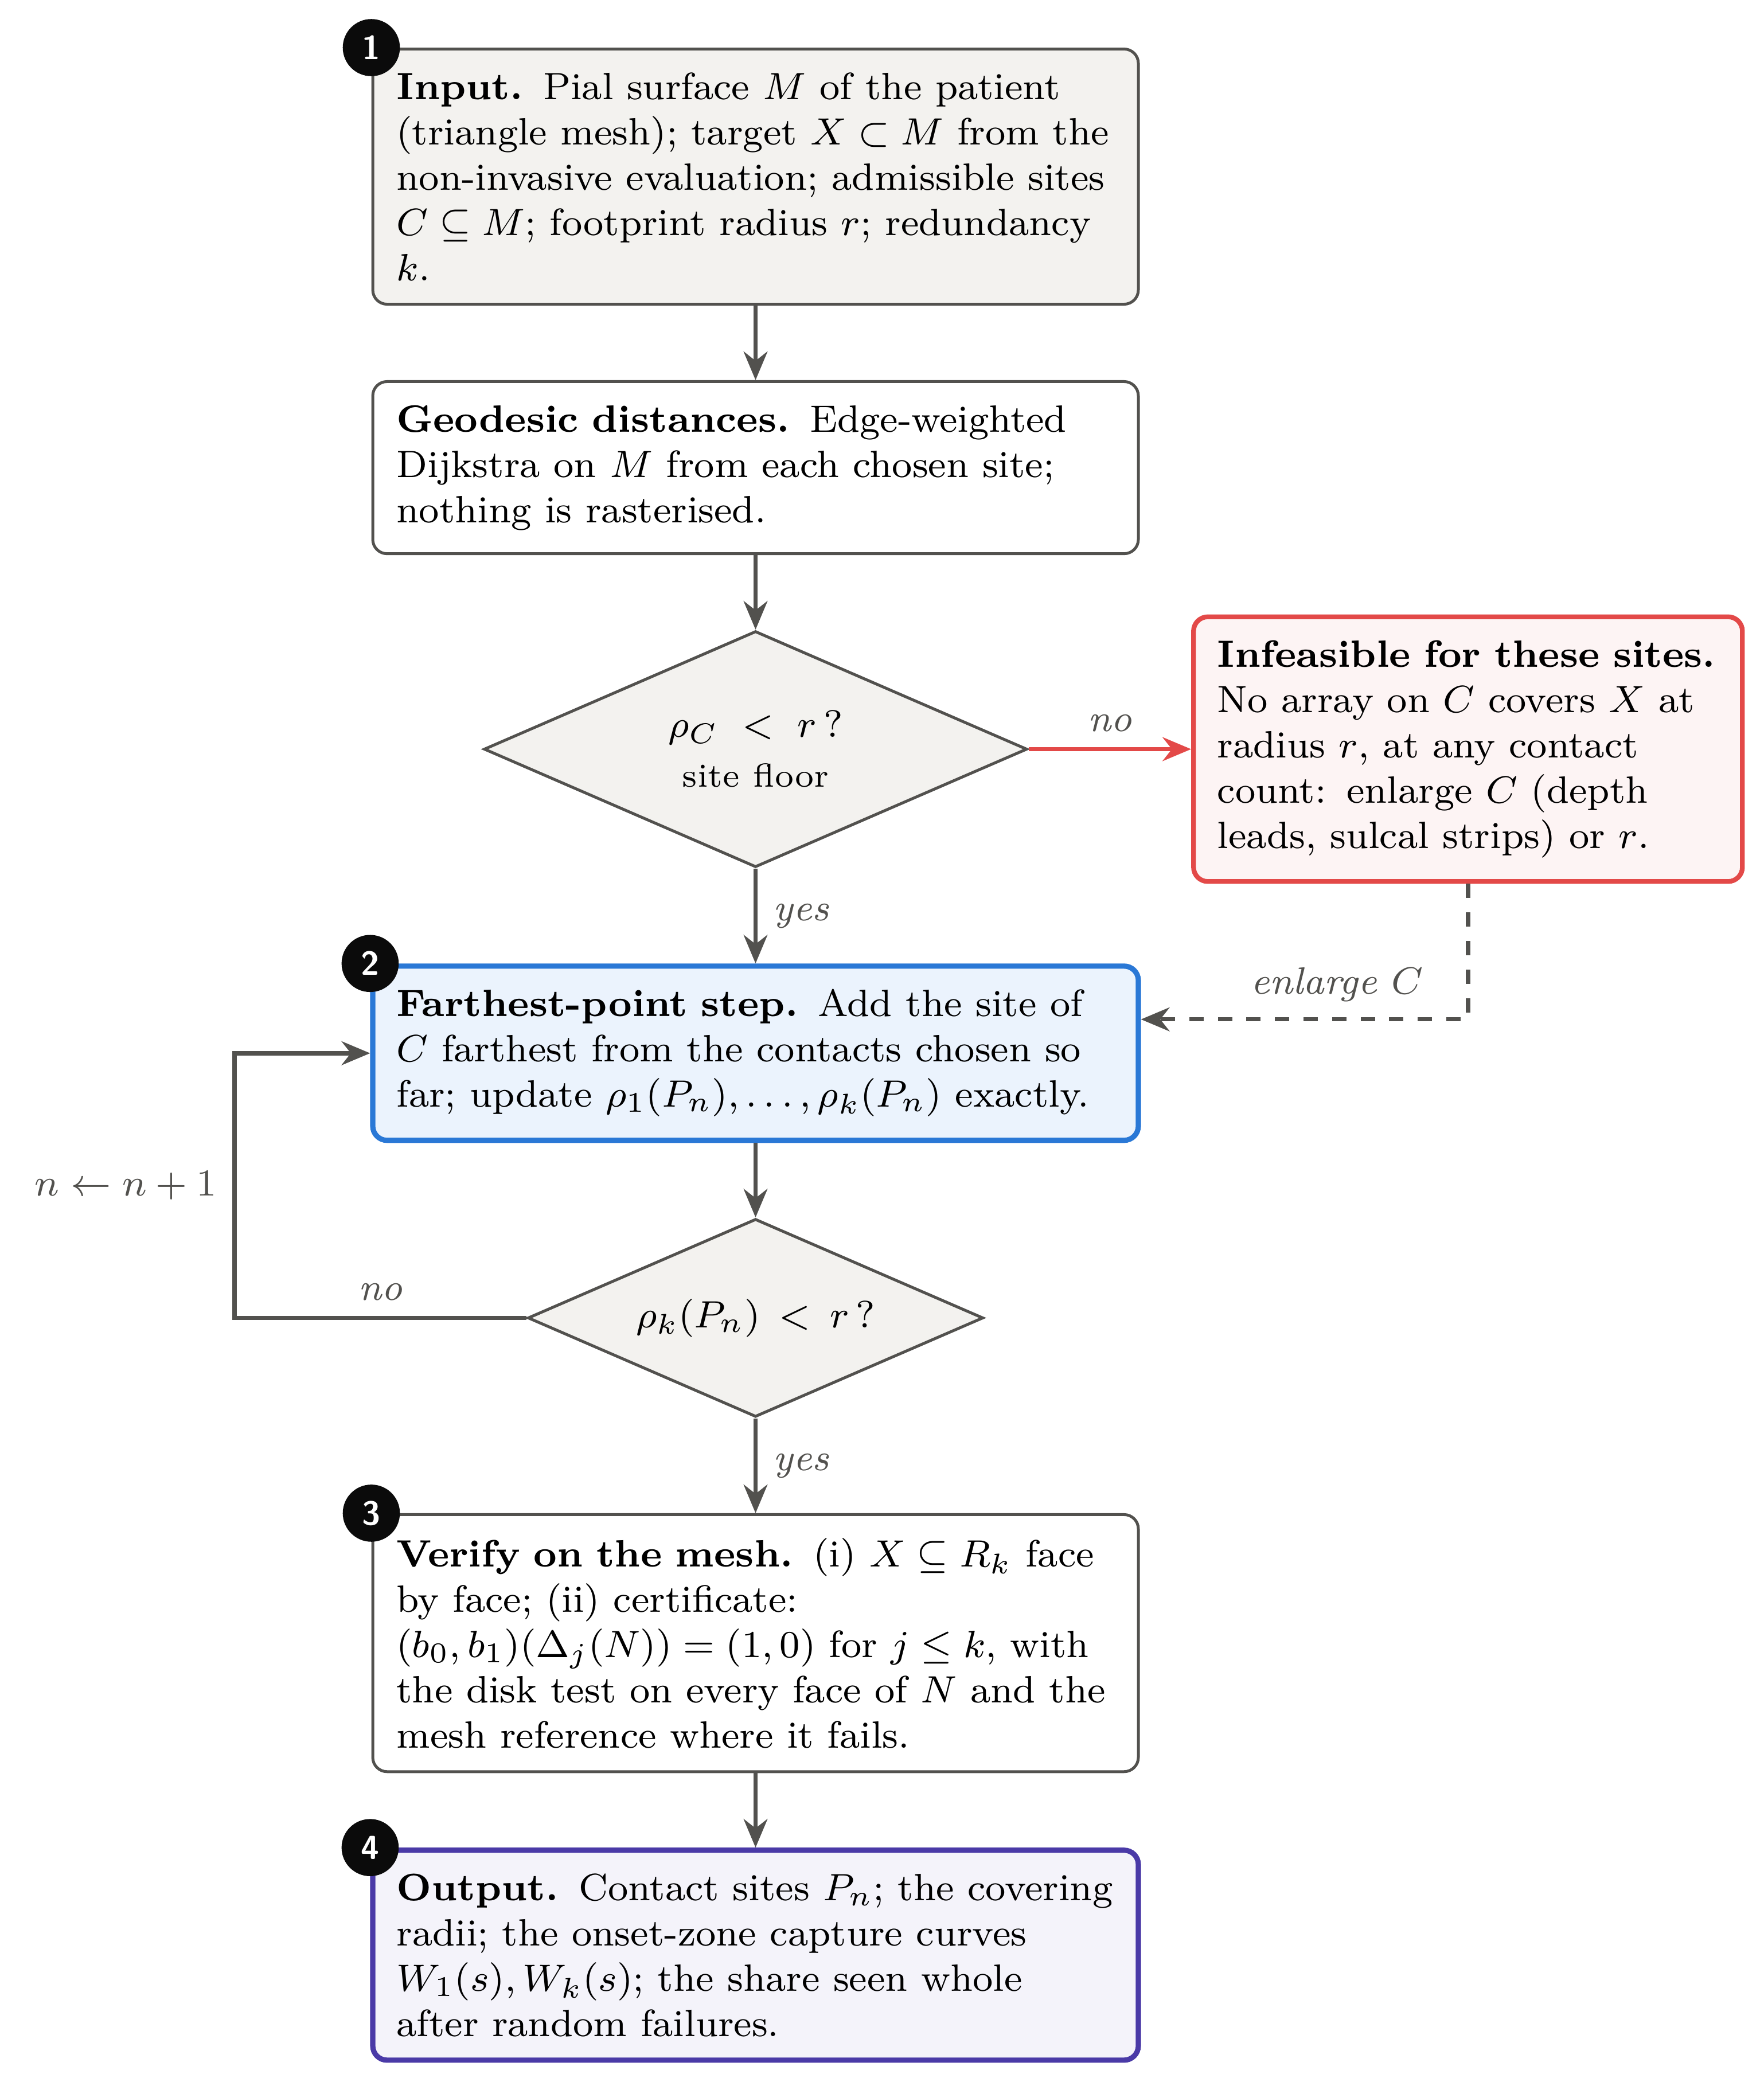
\includegraphics[width=0.62\textwidth]{fig4_algorithm.png}
\caption{The design procedure. The site-floor test
(Proposition~\ref{prop:sitefloor}, with the $k$-th nearest site) rules out,
before any placement, admissible sites that cannot see $X$ $k$ times at radius
$r$. Greedy steps add contacts until the $k$-th covering radius drops
below $r$ (Proposition~\ref{prop:cover}); for $k=1$ with sites anywhere on $X$
they are within a factor two of optimal, up to one mesh edge
(Proposition~\ref{prop:greedy}). The
design is then checked on the mesh and its onset-zone capture is reported
(Proposition~\ref{prop:erosion}).}
\label{fig:algorithm}
\end{figure}

% =====================================================================
\section{Results on a template cortex}\label{sec:results}
% =====================================================================

\subsection*{Surface and territory}
The surface is the left pial surface of the colin27
template~\cite{Holmes1998}, as distributed with FieldTrip~\cite{Oostenveld2011}:
$\meshVerts$ vertices and $\meshTris$ triangles, every edge in exactly two
triangles, Euler characteristic~2. The territory $X$ is every triangle within
$\patchRadius$\,mm, along the surface, of a parietal anchor at MNI
$\anchorMNI$: $\patchVerts$ vertices, $\patchTris$ triangles and
$\patchArea$\,mm$^2$, a topological disk. The reference array is the
$8\times8$ parietal grid of the FieldTrip ECoG tutorial layout~\cite{Stolk2018},
$10$\,mm pitch, transferred to the template by laying the lattice on the
envelope of the hemisphere and assigning each lattice point to the nearest gyral
vertex; its median neighbour spacing is $\gridEuPitchMedian$\,mm in a straight
line and $\gridGeoPitchMedian$\,mm along the surface, and $\gridOutsideX$ of its
64 contacts lie outside $X$. This is template geometry, not a patient's
implantation.

\subsection*{Where the contacts sit decides the coverage}
At $r=8$\,mm the $8\times8$ grid leaves $\gridUnseenEight$\,mm$^2$
($\gridUnseenPctEight\%$) of $X$ unseen, and its covered region, with Betti
numbers $(b_0,b_1)=\gridBettiEight$, is in pieces and has holes. The same 64
contacts placed by farthest-point sampling over $X$ leave
$\greedyUnseenEight$\,mm$^2$ unseen (Figs.~\ref{fig:cortex}
and~\ref{fig:designs}b). At $10$ and $12$\,mm the grid still misses
$\gridUnseenPctTen\%$ and $\gridUnseenPctTwelve\%$, and the placed array misses
nothing. The covering radius says why (Fig.~\ref{fig:covering}). The grid's
is $\capRhoOneGridEight$\,mm. The placed array's is $\rhoFreeSixtyFour$\,mm,
just above $8$\,mm, which is why $\greedyUnseenEight$\,mm$^2$ stays unseen;
$\minNOneEight$ contacts bring it to $\minRhoOneEight$\,mm and leave nothing.

\begin{figure}[t]
\centering
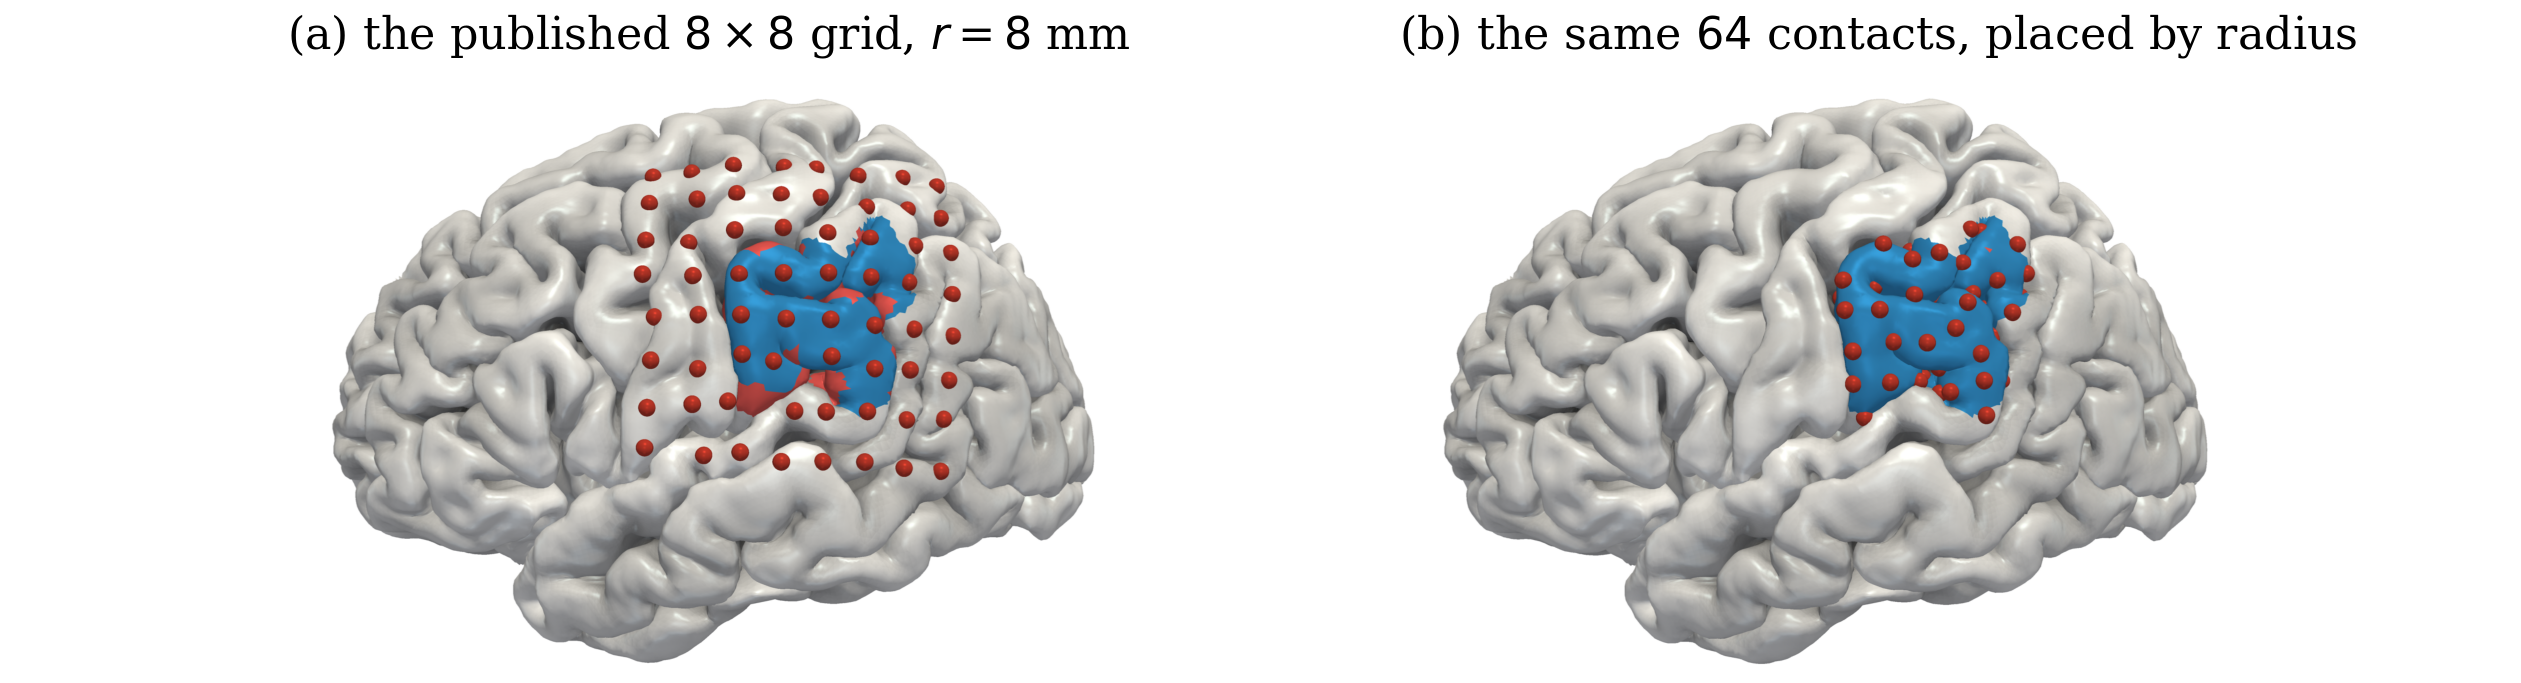
\includegraphics[width=\textwidth]{fig5_cortex.png}
\caption{The target territory $X$ on the colin27 left hemisphere at footprint
radius $r=8$\,mm, blue where some contact sees the cortex and red where none
does. (a) The documented $8\times8$ grid (red spheres), laid on the envelope of
the hemisphere: most of the unseen cortex lies on sulcal banks, hidden from
this view. (b) The same 64 contacts placed by covering radius. Rendered from
the repository's result files with PyVista.}
\label{fig:cortex}
\end{figure}

\subsection*{The site floor on real anatomy}
Take $C$ to be the gyral crowns, the vertices of negative sulcal depth, where
a sheet on the envelope puts its contacts. A sheet is not confined to the
crowns inside $X$, so we count every crown vertex within $\crownReach$\,mm of
$X$, $\crownSites$ of them; none farther can see any triangle of $X$ at the
radii that matter here. The site floor is $\rho_C=\crownFloor$\,mm, at a
triangle whose centroid is at MNI $\crownWorstMNI$, part way down a sulcal
bank, and $\rho_C^{(2)}=\crownFloorTwo$\,mm for double coverage. (On the
vertex rule the floor is $\crownFloorVertex$\,mm; counting only the
$\crownSitesInside$ crown vertices inside $X$ would give
$\crownFloorInside$\,mm.) A crown-only sequence, which at each step adds the
crown site closest to the worst covered triangle, reaches the floor at
$n=\crownFlatN$ and stays there (Fig.~\ref{fig:covering}). By
Proposition~\ref{prop:sitefloor}, no array with its contacts on the crowns
sees all of $X$ at a footprint radius at or below this floor, whatever
its pitch or contact count. With 64 crown contacts at $r=8$\,mm,
$\capUnseenCrownEight$\,mm$^2$ of $X$ stays unseen.

\begin{figure}[t]
\centering
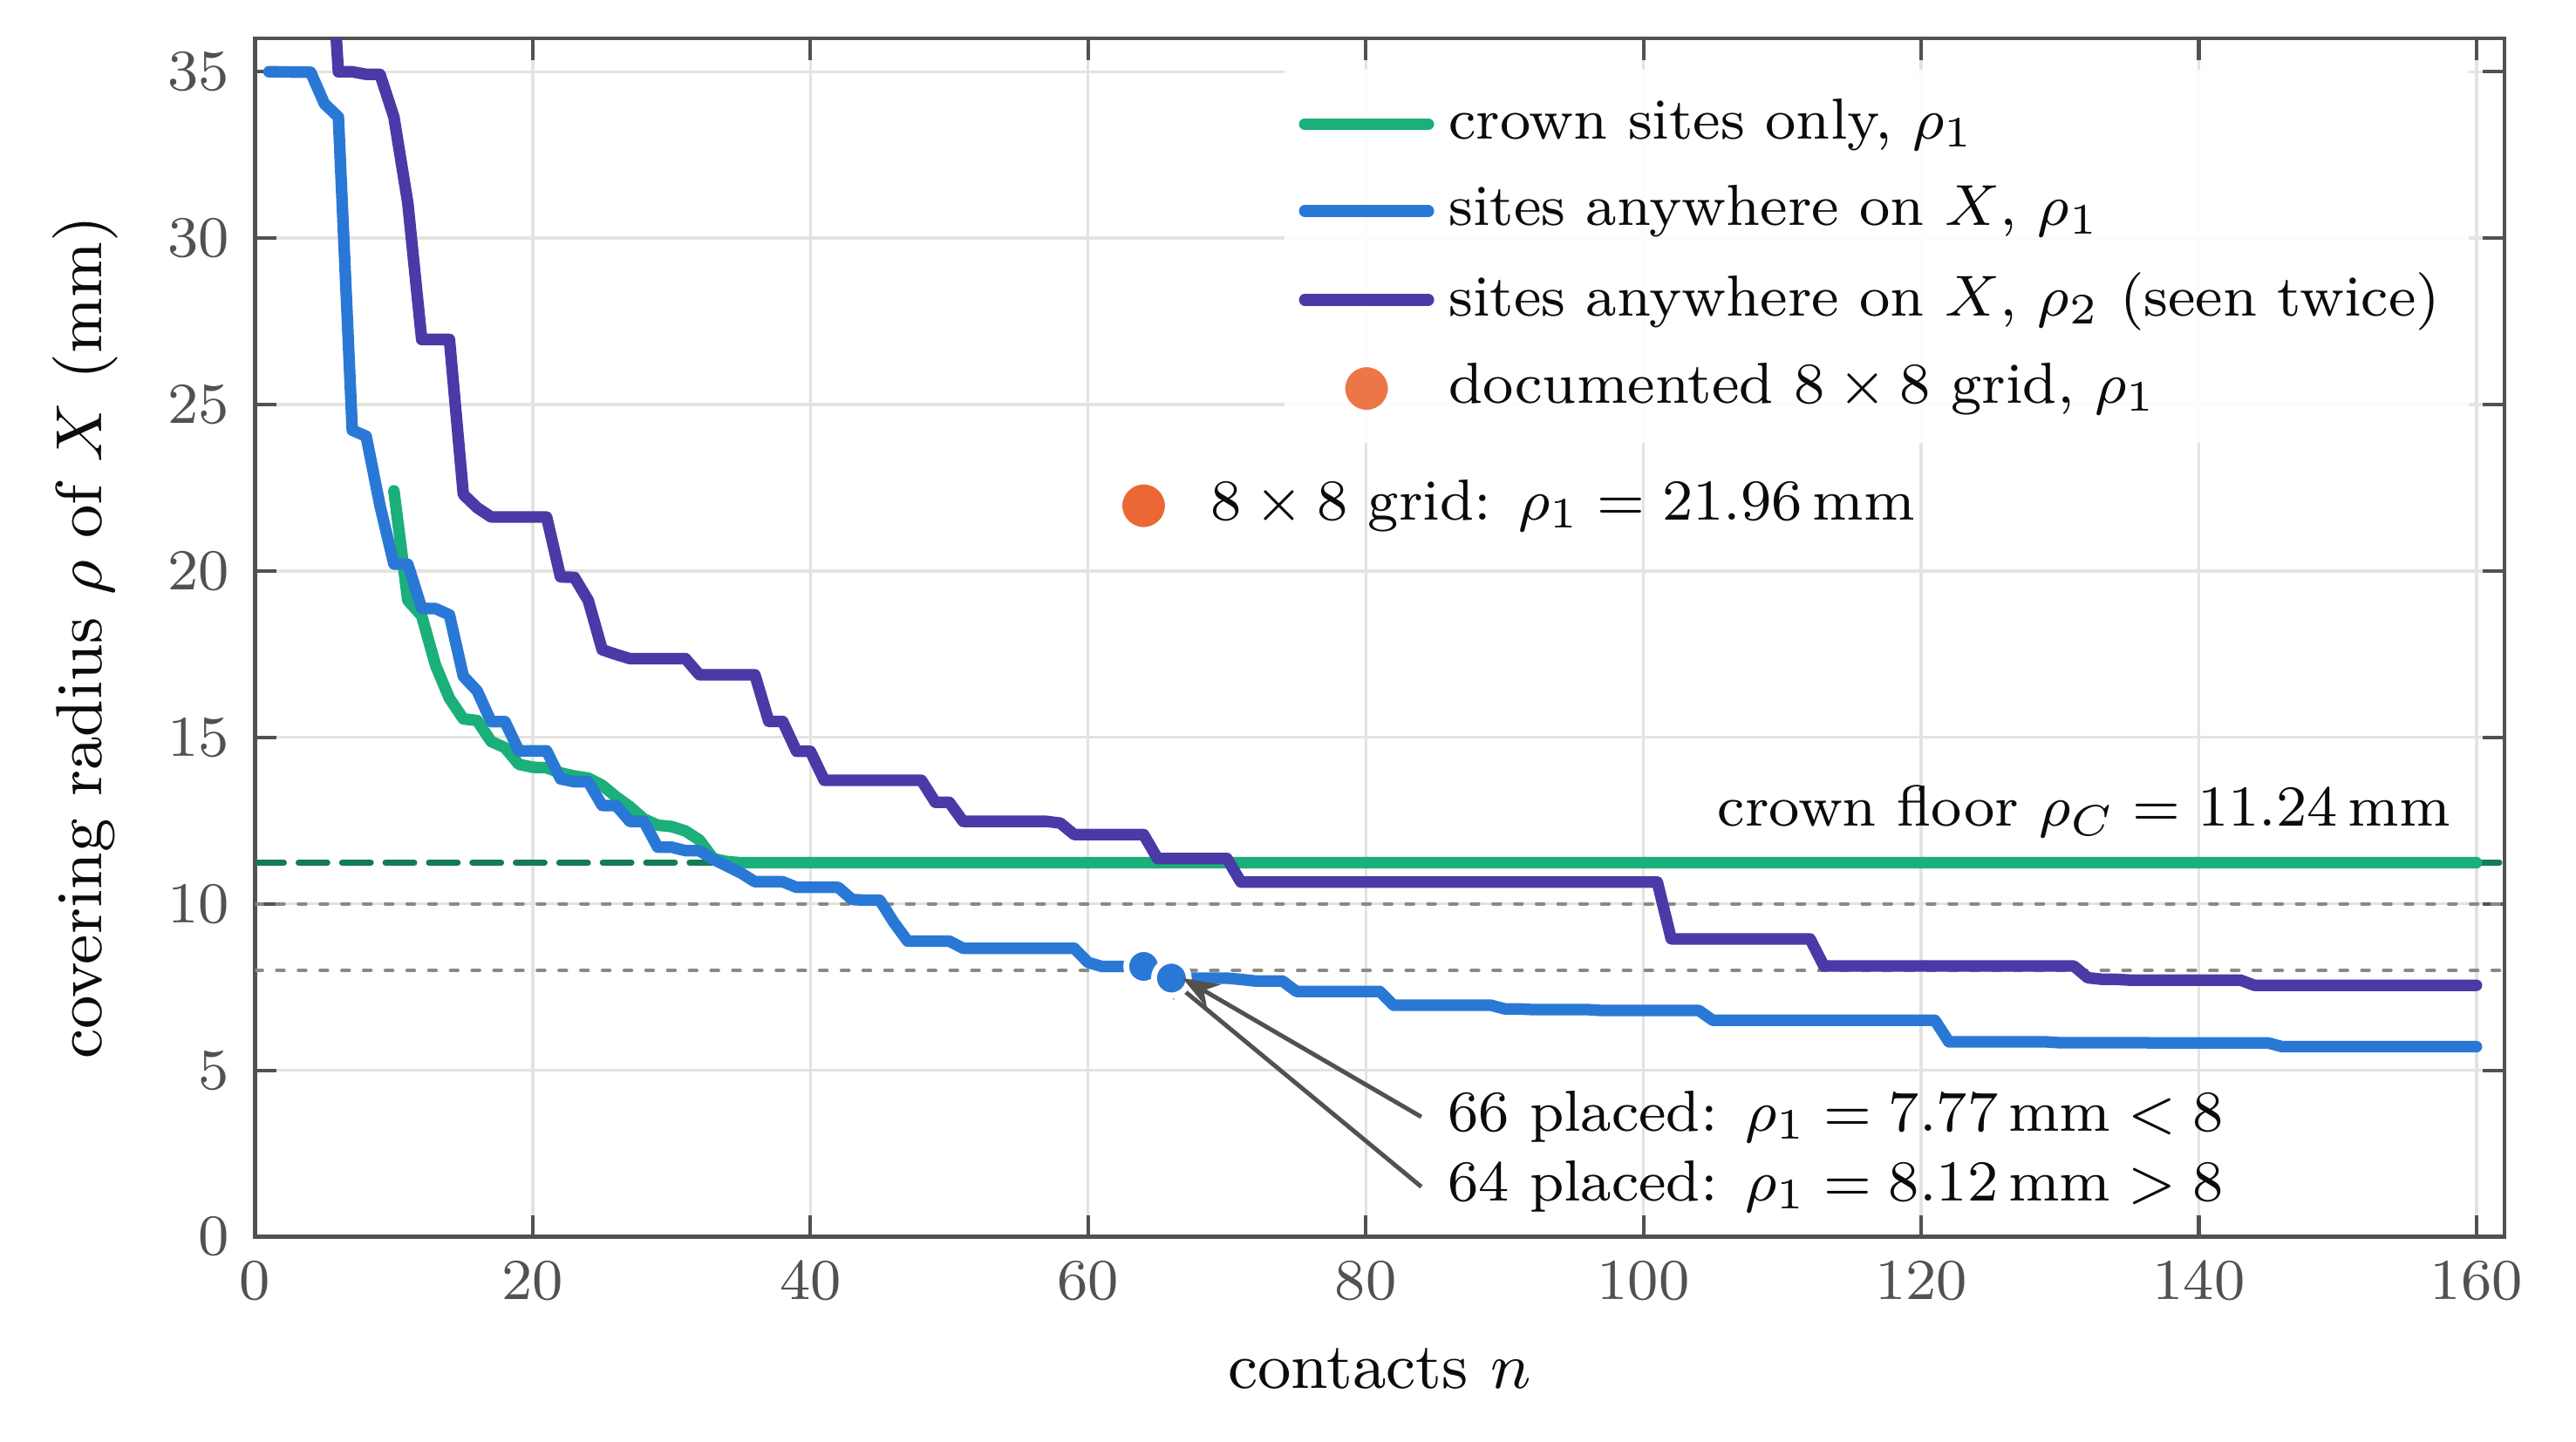
\includegraphics[width=0.82\textwidth]{fig6_covering.png}
\caption{Covering radius of $X$ against contact count, on the triangle rule.
Blue: sites anywhere on $X$, placed by farthest-point sampling. Green: sites on
gyral crowns within reach of $X$, which cannot fall below the crown floor
$\rho_C=\crownFloor$\,mm (dashed). Violet: the second covering radius $\rho_2$
of the blue sequence, which sets double coverage. Orange: the documented
$8\times8$ grid. Dotted lines mark $r=8$ and $10$\,mm; a design sees all of $X$
at radius $r$ exactly when its curve is below the line
(Proposition~\ref{prop:cover}).}
\label{fig:covering}
\end{figure}

\subsection*{How few contacts}
Table~\ref{tab:designs} gives, at each footprint radius, the fewest contacts of
the farthest-point sequence that see all of $X$ once and twice, found by
scanning one contact at a time; at every radius, one contact fewer leaves part
of $X$ unseen. Single coverage takes from $\minNOneFourteen$ contacts at
$14$\,mm to $\minNOneEight$ at $8$\,mm, against packing lower bounds of
$\packFourteen$ to $\packEight$, and double coverage from $\minNTwoFourteen$ to
$\minNTwoEight$ (Fig.~\ref{fig:designs}a). Every design below the crown floor
needs sites off the crowns: between $\offCrownPctLo\%$ and $\offCrownPctHi\%$ of
their sites lie in sulcal territory that a sheet cannot reach and a depth lead
or a sulcal strip can. The certificate agrees with the mesh for every
single-coverage design. For double coverage at $9$, $12$ and $14$\,mm the nerve
gives $(1,0)$ for $R_2$ while the mesh finds a hole in it; since all of $X$ is
seen twice, the hole lies outside $X$, and it is missed by the nerve because
geodesic footprints on a folded surface are not always convex. This is why
containment is always decided by Proposition~\ref{prop:cover} on the mesh.

\begin{table}[t]
\centering\small
\caption{Fewest contacts of the farthest-point sequence that see all of $X$
once ($k=1$) and twice ($k=2$), scanned one contact at a time, with their
covering radii (triangle rule), the Betti numbers of $R_k$ from the nerve and
from the mesh, and the packing lower bound for single coverage
(Proposition~\ref{prop:packing}).}
\label{tab:designs}
\setlength{\tabcolsep}{5pt}
\begin{tabular}{rrrccrrccr}
\toprule
 & \multicolumn{4}{c}{$k=1$} & \multicolumn{4}{c}{$k=2$} & \\
\cmidrule(lr){2-5}\cmidrule(lr){6-9}
$r$ (mm) & $n$ & $\rho_1$ (mm) & nerve & mesh & $n$ & $\rho_2$ (mm) & nerve & mesh & bound\\
\midrule
14 & $\minNOneFourteen$ & $\minRhoOneFourteen$ & $\minShadowOneFourteen$ & $\minMeshOneFourteen$ & $\minNTwoFourteen$ & $\minRhoTwoFourteen$ & $\minShadowTwoFourteen$ & $\minMeshTwoFourteen$ & $\packFourteen$\\
12 & $\minNOneTwelve$ & $\minRhoOneTwelve$ & $\minShadowOneTwelve$ & $\minMeshOneTwelve$ & $\minNTwoTwelve$ & $\minRhoTwoTwelve$ & $\minShadowTwoTwelve$ & $\minMeshTwoTwelve$ & $\packTwelve$\\
10 & $\minNOneTen$ & $\minRhoOneTen$ & $\minShadowOneTen$ & $\minMeshOneTen$ & $\minNTwoTen$ & $\minRhoTwoTen$ & $\minShadowTwoTen$ & $\minMeshTwoTen$ & $\packTen$\\
9 & $\minNOneNine$ & $\minRhoOneNine$ & $\minShadowOneNine$ & $\minMeshOneNine$ & $\minNTwoNine$ & $\minRhoTwoNine$ & $\minShadowTwoNine$ & $\minMeshTwoNine$ & $\packNine$\\
8 & $\minNOneEight$ & $\minRhoOneEight$ & $\minShadowOneEight$ & $\minMeshOneEight$ & $\minNTwoEight$ & $\minRhoTwoEight$ & $\minShadowTwoEight$ & $\minMeshTwoEight$ & $\packEight$\\
\bottomrule
\end{tabular}
\end{table}

\begin{figure}[t]
\centering
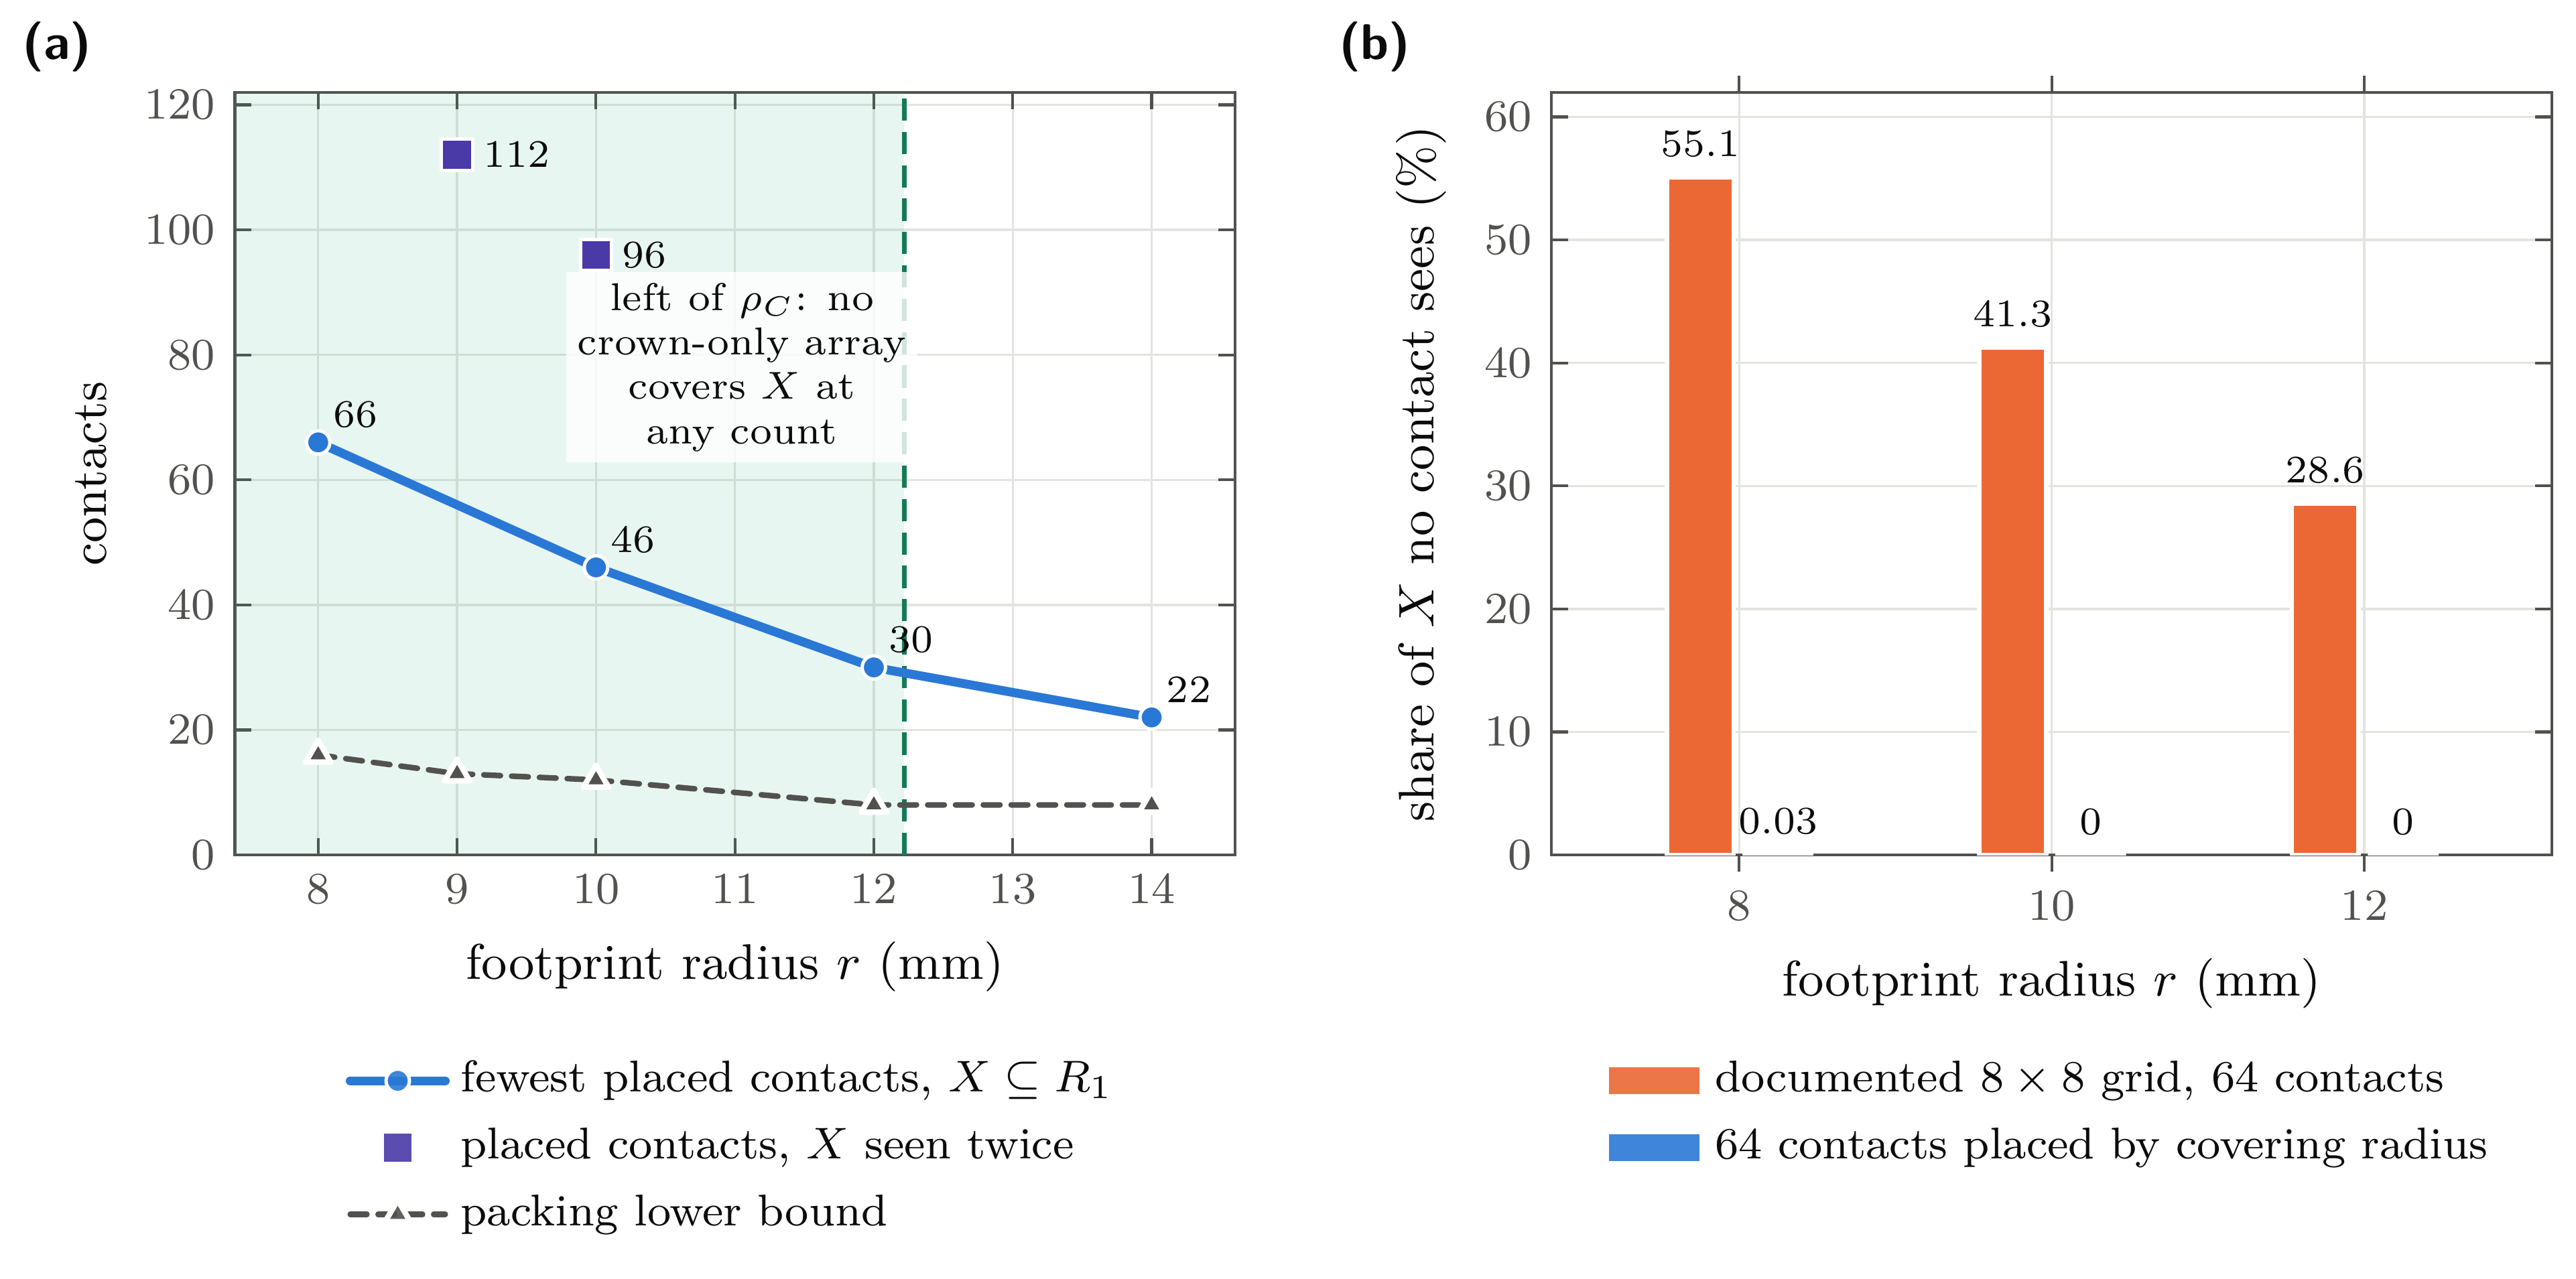
\includegraphics[width=\textwidth]{fig7_designs.png}
\caption{(a) Fewest contacts of the farthest-point sequence that see all of
$X$ once (blue) and twice (violet), against the packing lower bound for single
coverage (grey). Left of the crown floor (shaded) no array with contacts on the
crowns sees all of $X$ at any count. (b) The share of $X$ that no contact sees,
for the documented $8\times8$ grid and for the same 64 contacts placed by
covering radius.}
\label{fig:designs}
\end{figure}

\subsection*{Seeing the onset zone whole}
Table~\ref{tab:capture} and Fig.~\ref{fig:capture} give the capture of an onset
zone of radius $s$ placed uniformly in $X$. With the $8\times8$ grid at
$r=8$\,mm, an onset zone of radius $5$\,mm is seen whole in
$\capWholeFiveGridEight\%$ of its possible positions and missed entirely in
$\capMissFiveGridEight\%$; one of radius $10$\,mm is seen whole in
$\capWholeTenGridEight\%$, and one of radius up to $\capHiddenGridEight$\,mm can
lie in $X$ and be missed entirely. The lower bound of
Proposition~\ref{prop:erosion}(2), $\max_x\min\{\dd_1(x,P)-r,\,
\dd(x,M\setminus X)\}$, evaluated at the vertices of $X$, is
$\gridHideBound$\,mm.
Sixty-four crown contacts never miss a $5$\,mm onset zone entirely but see it
whole in only $\capWholeFiveCrownEight\%$ of positions: the rest are seen in
part, the case of truncated localisation. The same 64 contacts placed anywhere
on $X$ see it whole in $\capWholeFiveFreeSixtyFour\%$ of positions, the
remainder being the positions within $5$\,mm of the $\greedyUnseenEight$\,mm$^2$
they leave unseen, where an onset zone smaller than
$\capHiddenFreeSixtyFour$\,mm can even be missed. The $\minNOneEight$ contacts
that see all of $X$ see every onset zone of every size whole, as
Proposition~\ref{prop:erosion}(1) requires.

\begin{table}[t]
\centering\small
\caption{Covering radii and onset-zone capture of each design on $X$, on the
triangle rule. $W_1$: positions in which an onset zone of radius $s$ is seen
whole; $L$: missed entirely; $W_2$: seen twice, hence whole after any one
failure; $h$: radius of the largest onset zone that can be missed entirely.
Percentages of admissible positions, area-weighted.}
\label{tab:capture}
\setlength{\tabcolsep}{4pt}
\begin{tabular}{lrrrrrrrrr}
\toprule
design & $r$ & $\rho_1$ & $\rho_2$ & unseen & \multicolumn{2}{c}{$W_1$ (\%)} & $L$ (\%) & $h$ & $W_2$ (\%)\\
\cmidrule(lr){6-7}
 & (mm) & (mm) & (mm) & (mm$^2$) & $s=5$ & $s=10$ & $s=5$ & (mm) & $s=5$\\
\midrule
$8\times8$ grid, 64 & 8 & $\capRhoOneGridEight$ & $\capRhoTwoGridEight$ & $\capUnseenGridEight$ & $\capWholeFiveGridEight$ & $\capWholeTenGridEight$ & $\capMissFiveGridEight$ & $\capHiddenGridEight$ & $\capTwiceFiveGridEight$\\
$8\times8$ grid, 64 & 10 & $\capRhoOneGridTen$ & $\capRhoTwoGridTen$ & $\capUnseenGridTen$ & $\capWholeFiveGridTen$ & $\capWholeTenGridTen$ & $\capMissFiveGridTen$ & $\capHiddenGridTen$ & $\capTwiceFiveGridTen$\\
crown sites, 64 & 8 & $\capRhoOneCrownEight$ & $\capRhoTwoCrownEight$ & $\capUnseenCrownEight$ & $\capWholeFiveCrownEight$ & $\capWholeTenCrownEight$ & $\capMissFiveCrownEight$ & $\capHiddenCrownEight$ & $\capTwiceFiveCrownEight$\\
placed, 64 & 8 & $\capRhoOneFreeSixtyFour$ & $\capRhoTwoFreeSixtyFour$ & $\capUnseenFreeSixtyFour$ & $\capWholeFiveFreeSixtyFour$ & $\capWholeTenFreeSixtyFour$ & $\capMissFiveFreeSixtyFour$ & $\capHiddenFreeSixtyFour$ & $\capTwiceFiveFreeSixtyFour$\\
placed, $\capNOneEight$ ($k=1$) & 8 & $\capRhoOneOneEight$ & $\capRhoTwoOneEight$ & $\capUnseenOneEight$ & $\capWholeFiveOneEight$ & $\capWholeTenOneEight$ & $\capMissFiveOneEight$ & $\capHiddenOneEight$ & $\capTwiceFiveOneEight$\\
placed, $\capNTwoEight$ ($k=2$) & 8 & $\capRhoOneTwoEight$ & $\capRhoTwoTwoEight$ & $\capUnseenTwoEight$ & $\capWholeFiveTwoEight$ & $\capWholeTenTwoEight$ & $\capMissFiveTwoEight$ & $\capHiddenTwoEight$ & $\capTwiceFiveTwoEight$\\
placed, $\capNOneTen$ ($k=1$) & 10 & $\capRhoOneOneTen$ & $\capRhoTwoOneTen$ & $\capUnseenOneTen$ & $\capWholeFiveOneTen$ & $\capWholeTenOneTen$ & $\capMissFiveOneTen$ & $\capHiddenOneTen$ & $\capTwiceFiveOneTen$\\
placed, $\capNTwoTen$ ($k=2$) & 10 & $\capRhoOneTwoTen$ & $\capRhoTwoTwoTen$ & $\capUnseenTwoTen$ & $\capWholeFiveTwoTen$ & $\capWholeTenTwoTen$ & $\capMissFiveTwoTen$ & $\capHiddenTwoTen$ & $\capTwiceFiveTwoTen$\\
\bottomrule
\end{tabular}
\end{table}

\begin{figure}[t]
\centering
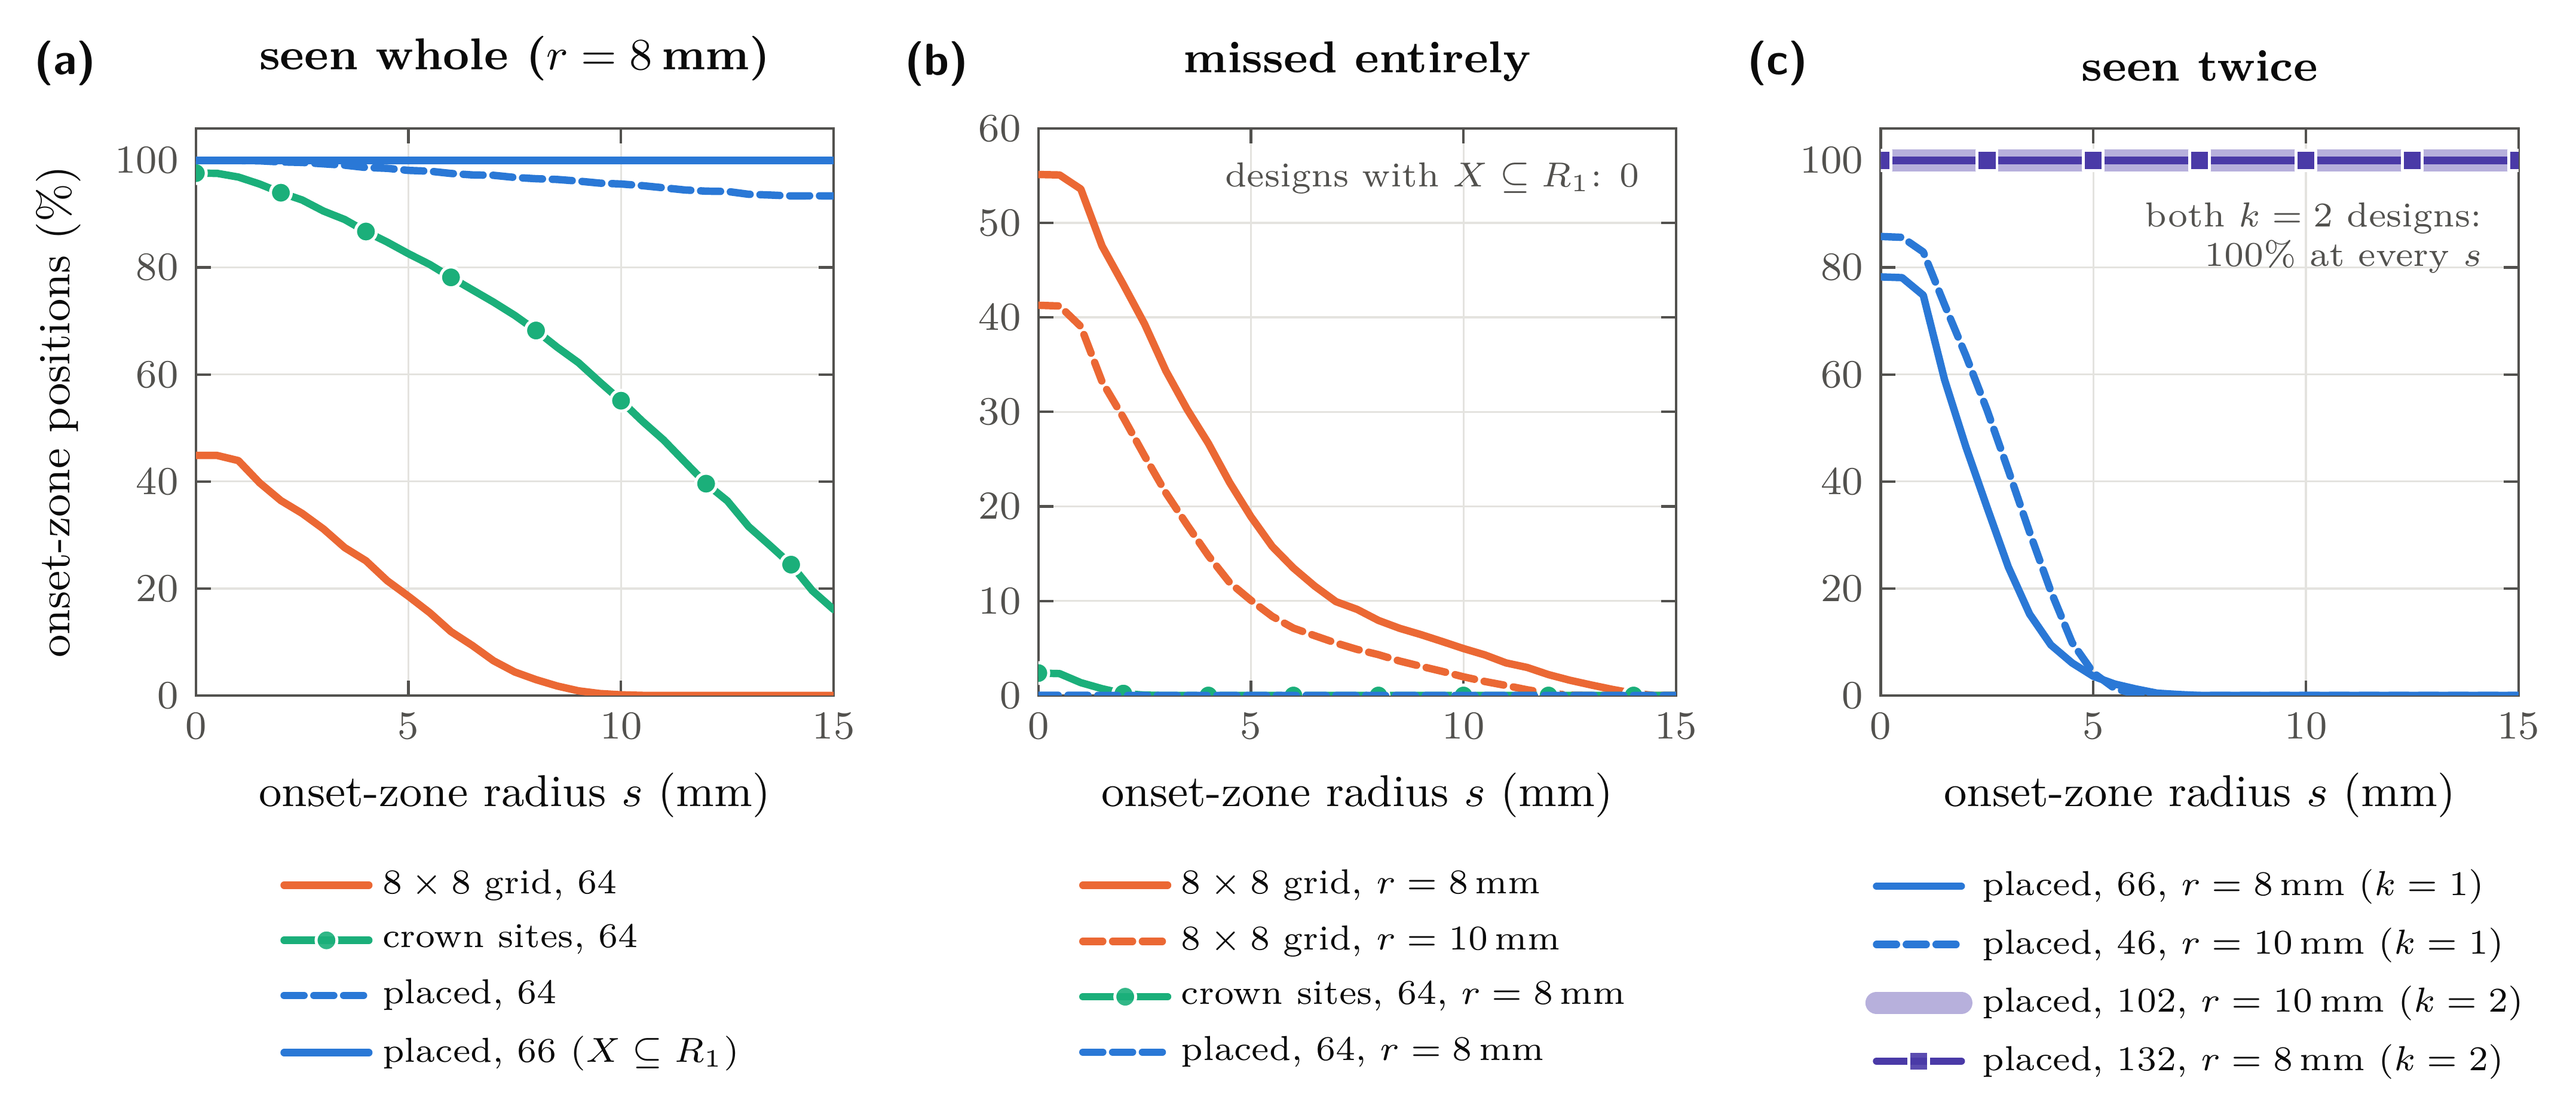
\includegraphics[width=\textwidth]{fig8_capture.png}
\caption{Onset-zone capture against onset-zone radius $s$, over all positions
in which the zone fits in $X$ (triangle rule; zones measured between triangle
centroids). (a) Seen whole, $W_1(s)$, at $r=8$\,mm: the $8\times8$ grid, 64
contacts on the crowns, 64 and $\capNOneEight$ contacts placed by covering
radius. (b) Missed entirely, $L(s)$; designs that see all of $X$ miss nothing,
and 64 placed contacts can miss only onset zones smaller than
$\capHiddenFreeSixtyFour$\,mm, too small to show. (c) Seen twice, $W_2(s)$,
which by Proposition~\ref{prop:failure} is the share still seen whole after any
one contact fails: single-coverage designs (blue) lose it quickly with $s$, and both
double-coverage designs (violet) keep it at $100\%$ for every $s$, so their
lines coincide. Data from
\texttt{run\_soz\_capture.py}.}
\label{fig:capture}
\end{figure}

\subsection*{When contacts fail}
Single coverage is fragile. The $\capNOneEight$-contact design sees a $5$\,mm
onset zone twice in only $\capTwiceFiveOneEight\%$ of positions, so one
well-placed failure can open a gap under most onset zones. Double coverage
repairs this: $\capNTwoEight$ contacts at $8$\,mm and $\capNTwoTen$ at
$10$\,mm see all of $X$ twice, $\rho_2=\capRhoTwoTwoEight$ and
$\capRhoTwoTwoTen$\,mm, and every onset zone survives any single failure.

Under random failure of $q$ contacts ($\dropDraws$ draws for each $q$), the
share of $5$\,mm onset zones still seen whole falls, for the
$\capNOneEight$-contact single-coverage design, to $\dropMeanOneOneEight\%$ at
$q=1$, $\dropMeanFourOneEight\%$ at $q=4$ and $\dropMeanEightOneEight\%$ at
$q=8$ (5th percentile over draws $\dropLowEightOneEight\%$). For the
double-coverage designs the lowest mean over all $q$ is $\dropMinTwoEight\%$ at
$8$\,mm and $\dropMinTwoTen\%$ at $10$\,mm (Fig.~\ref{fig:dropout}). The
$8\times8$ grid starts at $\capWholeFiveGridEight\%$ and ends at
$\dropMeanEightGridEight\%$. The price of failure-proof sampling is contacts:
$\capNTwoEight$ against $\capNOneEight$ at $8$\,mm, and $\capNTwoTen$ against
$\capNOneTen$ at $10$\,mm, which is the trade the design procedure makes
explicit.

\begin{figure}[t]
\centering
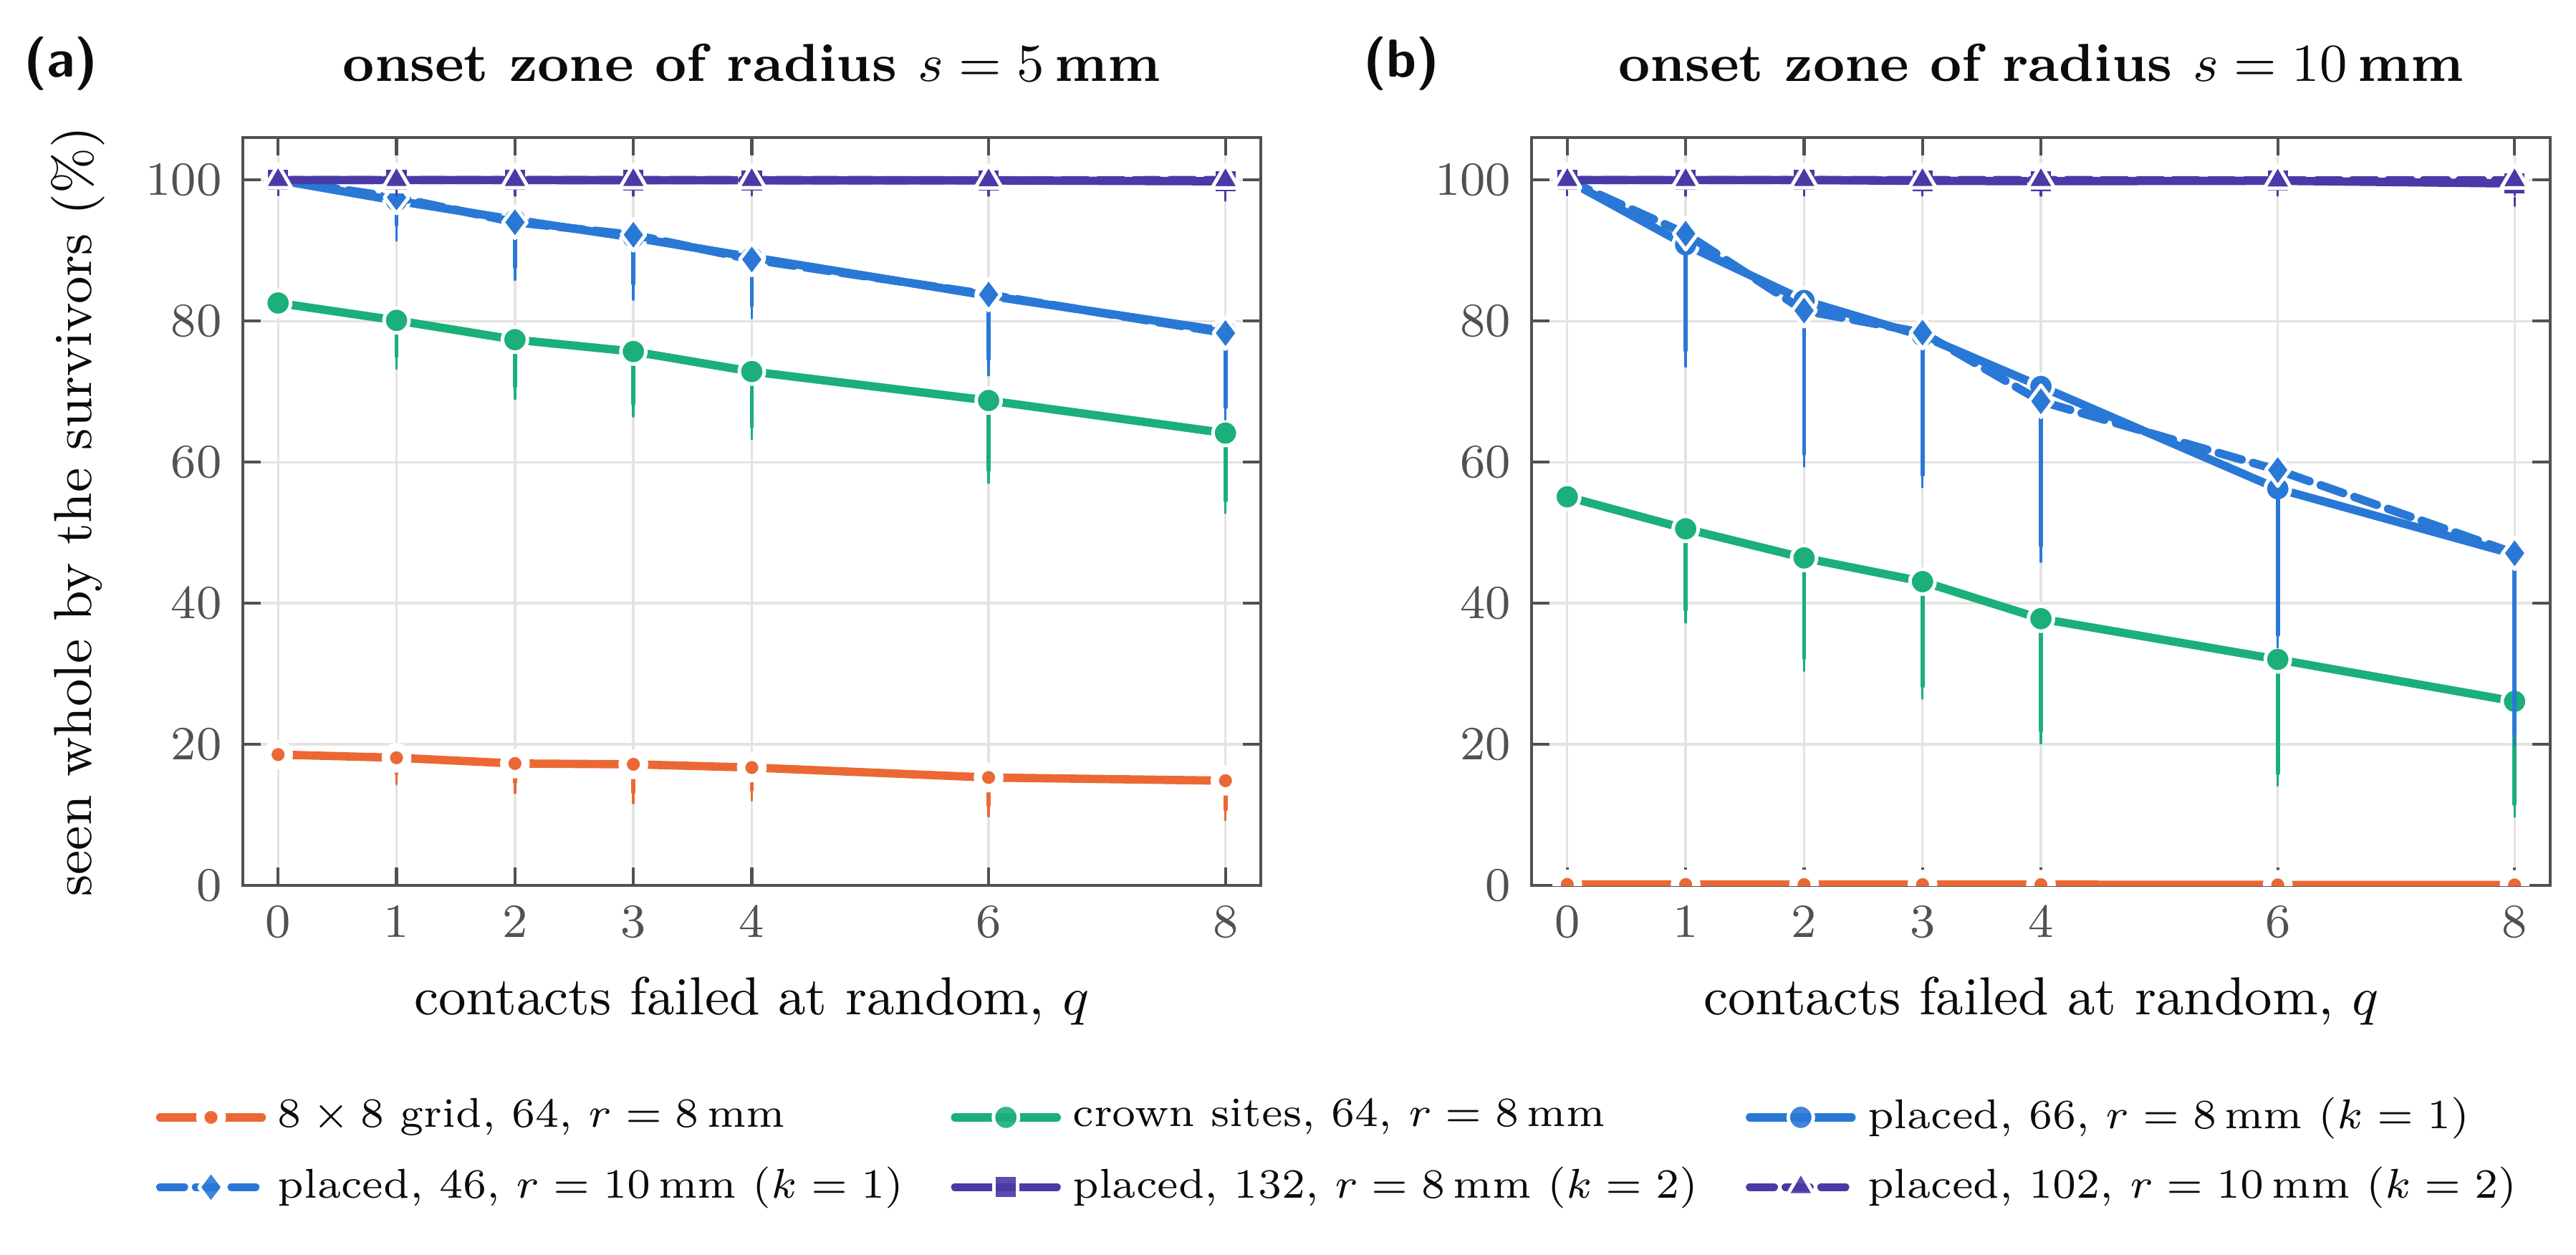
\includegraphics[width=\textwidth]{fig9_dropout.png}
\caption{Onset zones still seen whole when $q$ contacts fail at random, for
onset zones of radius (a) $5$\,mm and (b) $10$\,mm. Lines are means over
$\dropDraws$ random failure sets for each $q$; whiskers reach down to the 5th
percentile. Single-coverage designs ($k=1$, blue) degrade with every failure;
double-coverage designs ($k=2$, violet) stay near $100\%$ through eight
failures. The uniform failure model is an assumption; failures clustered in
space would be harder on every design.}
\label{fig:dropout}
\end{figure}

% =====================================================================
\section{Discussion}\label{sec:discussion}
% =====================================================================

\subsection*{What optimal coverage buys}
The results separate two things that ``coverage'' runs together: how many
contacts an array has, and where they sit. On this territory the documented
grid and a placed array with the same 64 contacts have covering radii of
$\capRhoOneGridEight$ and $\rhoFreeSixtyFour$\,mm, and differ by more than half
the territory in what they see. The covering radius explains the difference in
one number, predicts the largest onset zone an array can miss
(Proposition~\ref{prop:erosion}), and is cheap enough to optimise directly.
Pushing $\rho_k$ below $r$ gives a worst-case guarantee that no average-case
measure gives: every onset zone of every size in $X$ is seen whole, and stays
so after any $k-1$ failures (Proposition~\ref{prop:failure}).

The site floor explains why subdural sheets have limits that no pitch or
contact count removes (Proposition~\ref{prop:sitefloor}). Between
$\offCrownPctLo\%$ and $\offCrownPctHi\%$ of the contacts of the designs
below the floor sit in sulcal territory, so an optimal design for a folded
territory is in part a depth-lead design. Stereo-EEG and hybrid implantations
reach sulcal and deep cortex that subdural grids do
not~\cite{Jayakar2016,ParviziKastner2018}. The procedure here says, for a given
patient and territory, how much of the territory a sheet can see at all,
before anything is implanted.

\subsection*{What it does not buy}
Seeing the onset zone whole is a condition for localising it, and localising it
is a condition for resecting it. Neither is sufficient for seizure freedom.
The recorded onset zone may not be the whole epileptogenic zone, the territory
$X$ may be wrong, and eloquent cortex may forbid the resection. Whether better
coverage changes outcome is therefore an empirical question, and the published
evidence does not settle it: the completeness of resection of the recorded
onset zone was not associated with outcome in one cohort~\cite{Gascoigne2024},
while spatial perturbation of implantations has been proposed as a way to test
whether the epileptogenic zone was sampled at all~\cite{Jaber2024}.

\subsection*{A test of clinical relevance}
The test needs patients with four things together: the reconstructed pial
surface, the implanted contact coordinates, the resection and the surgical
outcome. Open intracranial datasets do not yet reliably provide all four.
OpenNeuro ds003029~\cite{Li2021}, for example, releases intracranial
recordings with clinically annotated channels and surgical outcome, but no MRI
or contact coordinates, which would have to come from the treating centres.
For each patient, compute on the patient's own surface the covering radius of
the resected territory by the implanted contacts, $W_1$ and $L$ over it, and
the same for the design this paper's procedure would have produced with the
same number of contacts. Then test, under a plan fixed before any outcome label
is read, whether coverage of the resected territory predicts seizure freedom.
A null result would bound the clinical value of optimal coverage. A positive
one would justify a prospective comparison of designed and conventional
implantations.

\subsection*{Limitations}
Everything here is computed on one template hemisphere and one territory, not
on patients. The footprint radius $r$ is a modelling parameter, the distance
along the cortex over which a contact is credited with recording an onset; it
is swept, not measured, and calibrating it from lead fields or from recorded
spread is the most important extension. Geodesic distance is shortest-path
distance on the mesh edges, which slightly overestimates the true surface
distance, and the triangle rule counts a triangle as seen only when one
contact sees all of it; both make the designs conservative by at most about
one mesh edge. Contact sites are mesh vertices, a site off the crowns stands
for a depth or sulcal contact without modelling its trajectory, and surgical
constraints (vessels, eloquent cortex, safe entry points) are not modelled;
they enter the procedure as a smaller site set $C$, which
Proposition~\ref{prop:sitefloor} then prices. The uniform priors over onset
position and over failures are assumptions. Failures clustered in space, as
real contact failures on scalp arrays have been found to be~\cite{kshadowcode},
would be harder on every design, and would reward coverage deeper than $k=2$.

% =====================================================================
\section{Methods}\label{sec:methods}
% =====================================================================

\subsection*{Surface and distances}
The left pial surface of colin27 is taken from FieldTrip at commit
\texttt{8e2307d}, in MNI millimetres; it is a de-identified reference anatomy,
not patient data. Distances are Dijkstra distances~\cite{Dijkstra1959} on the
edge graph with Euclidean edge lengths. A triangle belongs to the footprint of
a contact when all three of its vertices lie within distance $r$ of it; the
unseen area of $X$ is the area of its triangles in no footprint. Gyral
vertices are those of negative FreeSurfer sulcal depth.

\subsection*{Designs}
Farthest-point sampling starts from the vertex of $X$ nearest to the anchor and
adds, at each step, a vertex of $X$ farthest from the contacts so far. The
triangle covering radii $\rho_1$ and $\rho_2$ of every prefix of this sequence
are computed exactly from $e(p,T)$, and the fewest contacts of
Table~\ref{tab:designs} are the first prefixes with $\rho_k<r$. The crown floor
is computed from $e(c,T)$ for every crown vertex within $\crownReach$\,mm of
$X$. The crown-only sequence adds, at each step, the crown site with the
smallest $e(c,T^\ast)$ to the worst covered triangle $T^\ast$ that is not yet
at its own floor. Packing bounds come from a maximal $2r$-separated set of
vertices of $X$. The certificate is computed with the nerve of the footprints,
the Betti numbers of $\Delta_k(N)$ over GF(2), a disk test on every face of the
nerve, and a mesh reference for $R_k$ computed without the nerve, all as
in~\cite{kshadowcode}. The designs are \texttt{run\_ecog\_designs.py}, about
five minutes.

\subsection*{Capture and failure}
Every triangle centroid is added to the edge graph as a node joined to the
three vertices of its triangle. For each design, one multi-source Dijkstra run
from the centroids of the triangles of $X$ held by fewer than $k$ footprints
gives, at every centroid of $X$, the distance to $X\setminus R_k$; one from
the centroids of the seen triangles gives the distance to $R_1$; and one from
the centroids outside $X$ decides admissibility. By
Proposition~\ref{prop:erosion}, $W_1$, $W_2$ and $L$ follow by thresholding at
each $s$ from $0$ to $15$\,mm in steps of $0.5$\,mm, with triangle areas as the
measure. For contact failure, $q\in\{1,2,3,4,6,8\}$ contacts are removed
uniformly at random, $\dropDraws$ times for each $q$ with fixed seeds, the
survivors' footprints are recomputed, and $W_1$ is taken again at $s=5$ and
$10$\,mm. The analysis is \texttt{run\_soz\_capture.py}, about a minute.

\subsection*{Lean formalization}
The combinatorial content of the propositions on the mesh is proved in the
Lean~4 proof assistant~\cite{deMouraUllrich2021}, in the directory
\texttt{lean/} of the repository (core Lean 4.22.0 without libraries, built
by \texttt{lake build}). Contacts and triangles are elements of arbitrary
types, and the distances $e(p,T)$ and $\dd$ are functions to the natural
numbers, for instance in micrometres. Only their order is used, together with
the symmetry and triangle inequality of $\dd$ for
Propositions~\ref{prop:packing} and~\ref{prop:greedy}. The theorems are:
\begin{itemize}
\item Proposition~\ref{prop:cover} (\texttt{cover\_iff}): every triangle of
$X$ lies in at least $k\ge1$ footprints if and only if, for every triangle,
the $k$-th smallest of its distances $e(p,T)$ is below $r$;
\item Proposition~\ref{prop:failure} for distinct contacts
(\texttt{failure\_proof}, \texttt{zone\_failure\_proof});
\item the equivalence behind Proposition~\ref{prop:erosion} on the mesh: an
onset zone about a centroid consists of triangles of a given kind exactly when
every other triangle of $X$ is farther than $s$ from that centroid
(\texttt{capture\_by\_erosion});
\item Proposition~\ref{prop:sitefloor}, in its $k$-fold form
(\texttt{site\_floor}, \texttt{site\_floor\_k});
\item Proposition~\ref{prop:packing} (\texttt{packing});
\item the pigeonhole step of Proposition~\ref{prop:greedy}
(\texttt{farthest\_point\_core});
\item the per-contact bounds $\dd(v,p)\le e(p,T)\le\dd(v,p)+\ell$ for a
vertex $v$ of $T$, behind $\rho_k^{\mathrm{v}}\le\rho_k\le
\rho_k^{\mathrm{v}}+\ell$ (\texttt{le\_triDist}, \texttt{triDist\_le}).
\end{itemize}
Every theorem depends only on the standard axioms of Lean (propositional
extensionality, choice and the soundness of quotients), and no proof is left
open. Not formalized are the statements on the continuous surface, among them
the measure argument of Proposition~\ref{prop:erosion}(2) and its lower bound
on $h(P)$, and the separation property of the farthest-point sequence to which
the pigeonhole step is applied.

\subsection*{Figures}
Figures~\ref{fig:pathway}--\ref{fig:algorithm} and
\ref{fig:covering}--\ref{fig:dropout} are TikZ and pgfplots sources, drawn from
the result files by \texttt{make\_ecog\_paper\_data.py} and rendered at
600\,dpi; the colours are a single palette checked for colour-blind
separation, with markers and line styles as a second channel.
Figure~\ref{fig:cortex} is the PyVista render of the repository.

\section*{Data availability}
No patient data are used. The template surface, the designs (every contact by
mesh vertex and MNI coordinate) and all result files are in the repository
below.

\section*{Code availability}
\begin{sloppypar}
All code, result files and figure sources are in the GitHub repository
\codeRepo~\cite{kshadowcode}. The Python code of this paper
(\texttt{run\_ecog\_designs.py}, \texttt{run\_soz\_capture.py} and the
designs and certificates they build on), its result files and its figure
sources are release \codeRelease, archived on Zenodo at
\href{https://doi.org/\zenodoDOI}{doi:\zenodoDOI}. The Lean formalization in
\texttt{lean/} was added to the repository after that release. This
manuscript is \texttt{paper/ecog/ecog\_coverage.tex}, built by
\texttt{paper/ecog/build.sh}. Every number in it is a macro generated from the
result files.
\end{sloppypar}

\section*{Acknowledgements}
\begin{sloppypar}
The Python computations and the Lean~4 formalization of this paper were
carried out with the assistance of Claude (Anthropic). They use the code in
the GitHub repository \codeRepo{}, release \codeRelease{}, archived on Zenodo
at \href{https://doi.org/\zenodoDOI}{doi:\zenodoDOI}.
\end{sloppypar}

\section*{Author contributions}
The idea of certifying $k$-fold sensor coverage through iterated nerve
complexes was first developed by D.B.\ with
U.B.~\cite{BhattacharjeeBhattacharya2026}. A.B.\ extended it to electrode
arrays on the cortex. D.B., U.B.\ and A.B.\ wrote the code and carried out
the analyses together, and all three authors wrote the paper.

\section*{Funding}
None.

\section*{Competing interests}
None.

\bibliographystyle{amsplain}
\bibliography{refs_ecog}

\end{document}
